\documentclass[letter,12pt]{article} 

\usepackage[english]{babel}
\usepackage[protrusion=true,expansion=true]{microtype}  
\usepackage{amsmath,amsfonts,amsthm,amssymb}
\usepackage{graphicx}
\usepackage{setspace}
\usepackage{amsthm}
\graphicspath{ {images/} }
\renewcommand\qedsymbol{$\blacksquare$}

\newtheorem{theorem}{Theorem}

\begin{document}
\begin{titlepage}
\title{\uppercase{Analysis of Rummy Games: Expected Waiting Times and Optimal Strategies}}
\author{\uppercase{Christopher Finkle}}
\date{}
\maketitle
\vspace{8cm}
\begin{center}A SENIOR RESEARCH PAPER PRESENTED TO THE DEPARTMENT OF MATHEMATICS AND COMPUTER SCIENCE OF STETSON UNIVERSITY IN PARTIAL FULFILLMENT OF THE REQUIREMENTS FOR THE DEGREE OF BACHELOR OF SCIENCE\\
\end{center}
\begin{center}
STETSON UNIVERSITY\\
2017\end{center}
\thispagestyle{empty}
\end{titlepage}

\newpage
\begin{titlepage}
\tableofcontents
\end{titlepage}
\newpage
\listoffigures
\newpage

\begin{abstract}
\begin{center}
EXPECTED TIME TO VICTORY IN GAMES OF THE RUMMY FAMILY 
 
By 
 
Christopher Finkle 
\end{center}  
Advisor: Dr. Erich Friedman\\
Department: Mathematics and Computer Science\\
\smallskip

We will examine card games of the rummy family. Specifically, we will attempt to find the expected waiting time before a given hand goes rummy. This, in turn, will lead to the ability to make optimal decisions about which cards to keep and which to discard to reach rummy most efficiently. We will use the techniques of discrete probability and expected value to perform this analysis. It is expected that the project will have a strong computational component which will be carried out using appropriate software.  

Initially, the project will deal with artificially simplified games of the rummy family in order to idealize our core technique. We will, for example, consider a game of three-card rummy which is assumed to be played without an opponent and with replacement of discards in the deck. We will gradually modify these simplifying assumptions until we are capable of analyzing the sorts of rummy games which actually appear ‘in the wild’, time and memory allowing. Eventually, we hope that the optimal strategy for given variants of rummy will be explored, with an eye towards uncovering results which apply to all games of the rummy family. 
\end{abstract}

\section{Introduction}

\subsection{Background and Objective}
The ability of computers to ‘solve’ human games of skill has increased greatly in tandem with processing power. Simple games like Checkers have been completely solved by exhausting the game states to determine the optimal move to counter any choice made by an opponent, while algorithmic approaches have allowed computers to eclipse the skills of the world’s best Chess and Go players despite the games not being solved in the same sense as Checkers, or even solvable using the resources available to human society. While artificial intelligences (AIs) designed to play specific games have continuously improved their abilities in contests of pure skill, their prowess in games which incorporate elements of chance is less assured.
 
We seek to shed light on one such class of card games – those of the Rummy family. We believe it may be possible to probabilistically ‘solve’ certain types of Rummy game so that the best possible decision (i.e. the decision which minimizes the expected time to Rummy) for any game state is known. Such a ‘solution’ would not be a deterministic one like the solution of Checkers, but it could shed light on the nature of the game and suggest pathways to a humanbeating AI all the same. 
 
\subsection{Games of the Rummy Family}

The history of Rummy-like games stretches back centuries, perhaps even longer than the existence of the standard deck of playing cards itself. The earliest observed game with Rummylike features come from China, where the tile-matching game Mahjong and the card game Khanhoo appeared during the middle part of the second millennium. The lineage of Khanhoo  continued with the Mexican game Conquian, the predecessor to all subsequent Rummy-like games (Parlett, 1978). Today, Rummy variants number in the thousands, with the most common being Straight Rummy and Gin Rummy (though each of these in turn has many variants). A few familiar examples are Canasta, Rummikub, and Tonk. \\

The defining features of a Rummy-like game are its mechanic and its objective. The mechanic is known as “draw-and-discard” – on each turn, a player draws a set number of cards (usually 1) into his hand and then discards a set number of cards (also usually 1) from his hand. Sometimes it is possible to pick up the card which the opposing player has just discarded. In this manner, hands evolve into each other one card at a time. The objective, meanwhile, is known as melding. To meld is to lay down a collection of cards, either a set (three or four cards of the same rank) or a run (three or more cards of the same suit in sequence). On a given turn, cards which cannot be incorporated into a meld are known as deadwood. The combination of this mechanic and objective makes the Rummy family well suited for mathematical analysis, as there is only a single decision to make on each turn (which card to discard) and each decision must be made with a single well-defined goal in mind (melding). Indeed, while many variants exist which complicate the nature of melding with desynchronization and complicated scoring systems, we will focus almost exclusively on a variant called Straight Gin Rummy, in which a player can only go out if all of the cards in their hand can be incorporated into melds simultaneously, because this is mathematically speaking the simplest goal possible for a Rummy-type game.\\

Some of the Rummy Family’s rule variations are worth considering in more detail. One of the most basic concerns the treatment of Aces. Commonly, they are low-valued, which means that only runs like A23 are allowed. However, some players prefer to count them as low or high, making A23 and QKA runs valid. Another variant, attested as “Round-the-Corner” or “Continuity”Rummy is even more forgiving, allowing runs to wrap around through the Ace, e.g. KA2 (Gibson). The myriad symmetries present in Round-the-Corner Rummy make it especially amenable to mathematical analysis, as we shall see later. \\
 
\subsection{Expected Value and Expected Time}

The expected value of a discrete random variable is the probability-weighted average of all possible values. For a discrete random variable , the expected value will be the sum of the products of the possible values of X with their respective probabilities of occurring. We write\\

$$E(X) = \sum_{x} x P(X = x)$$

We are interested in the expected value of one variable, $Y$, relative to another random variable $X$.

\begin{theorem}

$$E(Y) = \sum_{x} E(Y | X = x) P(X = x)$$
\end{theorem}

\begin{proof}
Using the definition of expected value we write

$$E(Y) = \sum_{y} y P(Y = y)$$

We introduce X by noting that $P(Y=y)=\sum_{x} P(Y=y \cap X = x) $ for any given X. Substituting, we find that

$$E(Y) = \sum_{y} y \sum_{x} P(Y = y \cap X = x)$$

Rearranging gives us

$$E(Y) = \sum_{y} \sum_{x} y \frac{P(Y = y \cap X = x)}{P(X=x)} P(X=x)$$

The Law of Total Probability tells us that $\frac{P(Y=y \cap X=x)}{P(X=x)} = P(Y=y | X=x)$. Substituting yields

$$E(Y) = \sum_{x} \sum_{y} y P(Y=y | X=x) P(X=x) $$

And another application of the definition of expected value suffices to show that

$$E(Y) =  \sum_{x} E(Y | X = x) P(X = x)$$

\end{proof}

This result will form the basis for our analysis of expected times, as the expected time to rummy of a hand, $E(Y)$, will be given by the sum of the expected values of that hand given each card $x$ in $X$, the probability space of available cards. \\

Another calculation of interest is that of expected time. For this quantity, the simplest scenario to consider is a trial which will either succeed or fail with a certain probability. If each successive trial is independent of all the previous ones, we call the probability distribution of this trial geometric, and the variable which describes its outcome is a geometric random variable. Consider a geometric random variable with success probability . We wish to find the expected time to success.\\

\begin{theorem}
For a geometric random variable $X$ with success probability $p$, the expected time to success is $\frac{1}{p}$. 
\end{theorem}

\begin{proof}
Let $T(X)$  be the expected time it takes for $X$ to succeed. The probability that $X$ is successful on time step $n$ is $(1−p)^(n-1) p$. The value of such an outcome will be $n$, since that is the time it took to succeed. So, using our definition of expected value we write 

$$E(X) = \sum_{n=1}^{\infty} (1-p)^{(n-1)} p n = \frac{p}{1-p} \sum_{n=1}^{\infty} n (1-p)^n =
	\frac{p}{1-p} \frac{1-p}{[1-(1-p)]^2} = \frac{1}{p} $$

The penultimate equality comes from the known relation $\sum_{x=1}^{\infty} x r^x = \frac{r}{(1-r)^2}$. (Saeed, 2005). This result will be useful in verifying some of the simplest results achieved by our later approach.

\end{proof}

\subsection{Existing Literature}

 A survey of scholarly articles related to Rummy games reveals that a project like ours has not been attempted – or at least, if it has, it has not been published. However, attempts have been made to develop Rummy-playing Artificial Intelligences (AIs) using bottom-up techniques, rather than the top-down enumerative approach we intend to pursue. Specifically, we look to a paper by Kotnik and Kalita, who employed two different methods of machine-learning to develop a Rummy-playing AI (Kotnik \& Kalita, 2003). Their approach is decidedly, pointedly agnostic about the finer points of the game’s structure. The AI sees game states, decisions, and its own slowly-refined value function relating the two. “There is no knowledge of the rules of the game built into the value function. There is no notion of sequences, sets or deadwood.” The AIs built using the team’s machine learning (ML) techniques showed improvement relative to a random player, but they were still soundly beaten by humans. \\

While intriguing, this machine-learning oriented approach elides exactly those mathematical features of Rummy which we intend to investigate. While Kotnik and Kalita’s work may offer little illumination of our specific path forward, it does serve as a goal we ultimately seek to match. If it is possible to develop a mathematically-determined policy function for a rummy game, rather than a ML-determined one, then that development would be the holy grail of our research.  
 
\section{A Computational Approach}

\subsection{The Combinatorial Explosion of Rummy}

The problem of evaluating the expected time to rummy of a given rummy hand is one complex enough that even with the immense capabilities of modern computers, a brute force strategy is doomed to failure. Attempts to evaluate hands in a holistic sense are apt to induce a ‘combinatorial explosion’ – there are so many factors multiplying the complexity of the calculation that it rapidly becomes impossible to carry out via brute force.\\

The total calculation to find the expected value of a single hand would involve running through an unfeasibly large number of paths of possible cards and decisions – indeed, we would have to evaluate the expected value for every possible sequence of cards which might be given to us over the course of the game. For a typical game of ten-card Rummy played with a standard deck, this would entail finding the expected time to rummy for $\binom{42}{10}*32!$ possible arrangements of the remaining 42 cards (as our outcome can be affected by the subset of 10 cards which ends up in the second player’s hand and by the order of the remaining 32 cards in the deck which we will draw from during the game). Furthermore, we have no way of knowing which discard decision will be optimal at a given turn on a given path, so we will have to evaluate $11^{16}$ possible sets of discard choices for each of the paths (since the game can take up to 16 turns and on each turn we have a choice of 11 cards which can be discarded). Then we must recall that all of this was for a single hand – of which there are $\binom{52}{10}$ possible. All in all, to completely solve the game of 10-card Straight Gin Rummy would require us to perform expected value calculations on $2.81*10^{71}$ game states – a task which is clearly infeasible with even the highest-powered supercomputer.\\

Reducing the size of the hands fails to alleviate this problem – in fact, it makes the explosion worse. By putting more cards back in the deck, dealing with smaller hands increases the number of possible game states found by this method of calculation by orders of magnitude. 

\subsection{The Strategy of Dynamic Programming}

For problems of great complexity, a strategy which is often useful is the decomposition of one large problem into several smaller subproblems, whose solutions can then be stored and called upon as needed in a process known as memoization. In practice, applications of dynamic programming appear in problems of optimization (what is the highest-valued path through a grid of values?) or enumeration (how many ways can we create a value from a set of coins?). 

It is our hope that by employing the techniques of dynamic programming, the complexity of the problem of solving Rummy can be reduced greatly (though perhaps not greatly enough to put it into the realm of possibility on consumer-grade hardware). It is perhaps obvious where memoization may be applied in our process. The immense brute-force operation above would ultimately employ the formula in $Theorem 1.1$ by summing the expected values for a hand over the set of pairs of the possible sequences of future draws and the possible sequences of future decisions. The central insight which allows us to deploy dynamic programming techniques is that each combination of possible future card and possible future decision leads to exactly one of the $\binom{52}{10}$ possible hands. From a starting hands there are a mere 42 possible draws, each of which leads to 10 possible new hands. If we were to know the expected values of each of these hypothetical hands, we could choose the minimum expected value (E) possible for each card – and thus sum our probability over only 42 values, which is eminently feasible. The expansion of this technique to encompass every hand again brings difficulties of scale, but the reduction in complexity between $\binom{52}{10}∙\binom{42}{10} \cdot 32! \cdot 11^{16}$ and $\binom{52}{10}\cdot42$ is certainly noteworthy

\subsection{Introduction of Simplifying Assumptions}

The keen-eyed reader may note that our scheme does not entirely preserve the complexity of the task at hand. As far as a player of Rummy is concerned, she has more available knowledge than simply the contents of her hand – she also knows which cards have been discarded. To see why this matters, consider a hand in which the player possesses two complete melds totaling 7 cards, plus the 2$\heartsuit$ , the 2$\diamondsuit$ and the 3$\diamondsuit$. In this case, there are four cards - A$\diamondsuit$, 4$\diamondsuit$, 2$\spadesuit$ and 2$\clubsuit$ - which can complete the gin rummy and win the game in a single turn. At the start of the game, these cards are 4 out of 42 cards whose positions are unknown, and thus the probability of drawing any one of them is $\frac{2}{21}$. If she does not draw one of the four, her optimal strategy is to simply discard the newly-drawn card and return to her initial state. A naïve calculation of expected value using the result of Theorem 1.2 leads us to believe that for such a hand, $E=\frac{21}{2}$
 
 But now imagine that the player holds this hand not at the beginning of the game, but several turns in – and that she has seen each of the four cards which could provide her with Rummy discarded by her opponent, taking them out of circulation. Now, assuming those cards are out of circulation, her best strategy is undoubtedly to begin discarding the deadwood in favor of newlydrawn cards in the hopes that new potential Rummies will emerge. As paths are closed off by discarding, it is possible for a hand with a very low  at the beginning of a game to become no better than completely disjointed deadwood. In other words, for a given hand, E is not solely determined by the contents of the hand; it is also affected by the complete game state on a given turn. 
 
 To perform our expected value calculations for each hand for each game state would end up creating a problem of exactly the same complexity as our initial brute force strategy – dynamic programming would not help us at all. We need to be able to assume that expected value results we found for our hypothetical hands are still valid – despite the fact that there is by definition a change in game state as we proceed from one hand to another by taking a turn, since we have now discarded a card that was not discarded before. 

In order to get around this issue, we will quite simply ignore it for the time being. We feel that this is justified for several reasons. First, it is still of interest to know the expected value of all hands in the starting game state, which is what our dynamic programming approach will most easily be able to calculate. Second, once our model is complete it should be possible to tweak it to calculate the best decision for any given non-starting game state in roughly the same amount of time that it takes to calculate for the starting game state (perhaps less!). The problem is not that calculating E for a given hand and game state is impossible, it is that there are so many game states that enumerating all of them beforehand is impossible. The final reason, however, is perhaps most compelling – in many games of Rummy, a card, once discarded, is not actually out of the game forever. So long as neither player wins within 16 turns, the discard pile will be shuffled, turned over, and used as the draw pile. In effect, this means that there is a constant churn of cards over a long enough time scale. The situation for our hypothetical player above is not quite as hopeless as it seemed, and she can still hope that one of the four cards will arrive – she just knows that it will take a bit longer. Over the vast array of possible game states, we conjecture that the temporary ‘out of circulation’ effect of discards will mostly be a wash, though of course this is a rich area of potential future investigation. 

For all these reasons, we will now introduce a vastly simplifying assumption that makes our dynamic programming approach work at all: we assume that after being discarded, each card is placed directly back into the deck (again, this effect occurs in actual games, just less uniformly). Furthermore, we treat our opposing player’s hand as an extension of the deck, since we have no way of knowing which cards are in which – in other words, we ignore the opposing player entirely for the time being.  

The fact that the player is a cipher who places discards directly back into the deck facedown means that we clearly cannot pick up our opponent’s discard. This reduces the number of decisions the player makes each turn from two to one. We may reintroduce this mechanic later, but for now it does not factor into our calculations. After all, the decision whether or not to choose the discard is based on whether its expected value is better than the expected value of a random draw, which is the very thing we seek to analyze in the first place. The knowledge of whether it is optimal to draw the discard will be predicated on our initial findings which ignore that same mechanic. With these assumptions in place, we are free to begin our exploration of how dynamic programming applies to games of the Rummy family.

\subsection{The Bellman Equation}
The Bellman equation, named for its inventor Richard Bellman, is a recursive functional equation which serves as a mathematical formulation of the technique of dynamic programming as it relates to optimization. Bellman’s approach relies on a form of ‘backward induction’ – starting with best of all possible outcomes, repeated application of the Bellman equation allows one to reason out the best decision possible for each preceding time step until some arbitrary ‘starting’ state is reached. In order to make its decision at each time step, the Bellman equation relies upon an objective value function $V(x)$ which must somehow be optimized for a state $x$. 

Bellman’s formulation relies on a number of other functions as well. What follows is an informal tour of the equation as it is ultimately derived; its recursive form is intuitive even without first seeing the derivation that rigorously proves its validity (Bellman, 1957).  

First, there is the decision function $\Gamma(x) = \{a_1,a_2,\ldots,a_n\}$, the set of decisions available from the state $x$. Each decision we can make will send us to a new state, in a process governed by the transformation function $T(x,a)$. It is here that we introduce recursion, for this new state will have its own value function, which we can find using $V(T(x,a))$. In some situations, we will care less about the value of each successive future generation, a quality of the decision making process known as impatience. When our decision-making process is impatient, we multiply the future value by a discount factor $0 < \beta< 1$. But what are these future values being discounted against? That would be the immediate payoff function $F(x,a)$, which tells us how our value function will change immediately should we make decision $a$ in state $x$. Because its consequence is immediate and unavoidable, it has no discount factor.

Let us put all of this together. Recall that we are seeking to optimize the value of $V(x)$. For the general case, let us assume that this means maximizing it. What are we maximizing? The values of outcomes, both present and future, as determined by decisions. The functions above describe how we find those outcomes. So, we write: 

$$V(x) = \max_{a \in \Gamma(x)}\{F(x,a)+\beta V(T(x,a))\}$$

This is the recursive formulation of the Bellman equation. While its notation may be abstruse at first, it does an excellent job of formalizing what at first seem to be strictly intuitive or qualitative notions about choice and value. It also happens to be simultaneously more general and less flexible than we need it to be to break down a Rummy game. We can now set about tinkering with its structure to suit our needs. 

\subsection{Modifying the Bellman Equation to Describe Rummy}

Perhaps the most obvious change is this: the optimization of our value function for a given hand will entail minimizing, rather than maximizing, the time to Rummy. So, with little change in the actual meat of the equation, we will write $V() = \min_{a \in \Gamma(x)}\{F(x,a)+\beta V(T(x,a))\}$. The mechanics of the game affect the equation as well. In non-Gin games, where melds can be laid down before the end of the game, an impatient decision process might make sense. However, the optimal decision-making process for Gin Rummy is patient – there is no payoff possible until the game ends, so our current turn ought not be privileged over future turns. They all contribute to our value function equally. When the decision making process is patient, we let $\beta= 1$, ultimately ignoring it. 
 
The deferred reward of Rummy greatly simplifies our immediate payoff function as well. $F(x,a)$ takes a game state and a decision, which in our case will be which card to discard. No matter what, discarding a card will complete a turn, thus increasing $V(x)$ by precisely 1. Even if the decision allows the player to go Gin, he has still taken one turn to do so. This simplicity of the payoff structure lets us define $F(x,a) = 1 \forall x \forall a$, which means in practice that we can replace it with the constant 1 in all cases. With these substitutions in place, we can now write a more specific version of the Bellman equation:

$$V(x) = \min_{a \in \Gamma (x)} \{1+V(T(x,a))\}$$

It is clear from our strategy that the game states x are in fact just stand-ins for hands h. In fact, we might as well just refer to our game states by the hand they entail, such that we write$V(x) = E(h)$. Now we can attempt to marry our understanding of expected value with our understanding of the Bellman equation, to find a formula which encompasses the stochasticity and determinism of the game, the draw and the discard (in that order). 

We are concerned with the value function $E(h)$ of an $n$-card hand $h$ consisting of cards $\{h_1,h_2,\ldots,h_n\}$. On our turn, there is a random distribution of cards which can be drawn, $X$, which contains each card not in $h$, all weighted with equal probability. In Theorem 1.1, we use the notation $E(Y | X = x)$ to mean the expected value of a variable $Y$ given a predetermined outcome for another variable $X$. We wish to convey a similar sentiment for our draw-dependent functions in the Bellman equation: what choices are available from a hand $h$ after we have drawn a card $x \in X$? What transformation function will tell us the results of this decision? The $(h | X=x )$ notation is cumbersome, so we will employ a different notation to indicate that it is given that $X=x$ . We will say that a given $x \in X$  will provide us with a set of possible actions $\Gamma_x (h) = \{a_0,a_1,\ldots,a_n\}$, where decision $a_k$ is the action of discarding $h_k$ if $0 < k \leq n$  and discarding the new card $x$ if $k=0$.

Finally, we can similarly define $T_x(h,a)$ to be the $n$-card hand that results from making decision $a \in \Gamma_x(h)$ with hand $h$ and new card $x$. Note that for any $x$, $h$, and $a$, $T_x(h,a_0)=h$. Since the value which we are optimizing is expected value, we can draw on Theorem 1.1 and rewrite it as: 

$$E(h) = \sum_{x \in X} \min_{a \in \Gamma_x (h)} \{1 + E(T_x(h,a))\} P(X = x)$$

\subsection{Iterating Over the Set of Hands}

Intuitively, since there is a deterministic $E(h)$ for each hand $h \in H$, we should be able to apply partial order to $H$ using $E$. Specifically, we say that $h_1 \leq h_2$ if $E(h_1) \leq E(h_2)$.

\begin{theorem}
For a hand $h_0 \in H$, $E(h_0)$ is determined only by the values of the hands in the set $\{h \in H | h < h_0\}$.
\end{theorem}

\begin{proof}
We will use induction. For our base case, consider the hands $\{h \in H | h \textrm{ is Rummy}\}$. By the rules of the game, we can end the game before even taking a turn, so $E(h) = 0$ regardless of our decision making structure.

Now, assume that there is some $n$-card hand $h_0$ for which we know all expected values $E(h)$ for values of $h$ in the set $\{h \in H | h < h_0\}$. We wish to show that our modified Bellman equation can determine $E(h_0)$ using only this information. Since our equation is a sum, we seek a way to reduce each term of the sum either to a constant or a term of order $E(h_0)$. If this can be achieved our equation will be linear and of one variable, and thus easily solvable.

This means that for each card $x \in X$, we need to know the value of 

$$\min_{a \in \Gamma_x (h_0)}\{1+E(T_x(h_0,a))\} P(X=x)$$

either as a constant or in terms of $E(h_0)$. $P(X=x)$ is always a constant multiplier, so we merely need to establish the value of the $min$ function. For a given card $x$, there are two possible cases. If it is possible for the card to improve our hand, then the value of the $min$ function is a known constant - since any improvement will have a lesser $E$, it will previously be known according to the Inductive Hypothesis.

The other case is that $x$ does not improve our hand. No matter what we discard, the resulting hand will be no better than $h_0$. Since $T_x(h_0,a) \geq h_0 \forall a \in \Gamma_x (h_0)$, it follows that $\min_{a \in \Gamma_x (h_0)}\{1+E(T_x(h_0,a))\} = 1 + E(h_0)$, a value which can always be achieved by taking $a_0 \in  \Gamma_x (h_0)$, which as noted above, will result in $T_x(h_0,a_0)=h_0$. If this is the case, the value of the $x$ term of the sum will be $P(X=x)(1+E(h_0)) = P(X=x) + P(X=x)E(h_0)$, which are a constant and a term of order $E(h_0)$ as desired.

Thus, no matter what, our equation can be made to consist of one variable, allowing it to be solved using only information about hands with lower $E$. The inductive step has been achieved. Starting from those hands which are Rummy, we can always solve for those hands with the next-smallest $E$ using only smaller $E$s, a process which will eventually find $E(h) \forall h \in H$
\end{proof}

With the theoretical proof that our approach works finally in place, we now turn to the practical. The ugly truth is that this calculation, evaluating each term of the Bellman sum using the knowledge we have, reducing it to the smallest known value or $1+E(h)$, and then solving the equation for $E(h)$, can be performed for any $h \in H$ regardless of whether the expected value of each member of $\{h \in H | h < h_0\}$ is known. Additionally, without foreknowledge of the value of $E(h_0)$, we cannot actually know whether $\{h \in H |h < h_0\} \subseteq \{h \in H | E(h) \textrm{ known}\}$ before we evaluate the Bellman sum. (That the converse is true follows from the recursive structure of our solution – since we must know all lesser $E$s to determine an $E$, it follows that at a given solution step all known $E$s are less than all unknown $E$s). Since the foreknowledge of $E$ for all members of $\{h \in H | h < h_0\}$ was a precondition for finding a valid result according to Theorem 2.1, this presents something of a problem. 

Fortunately, there is a way to figure out after the fact whether our solution for a given hand is accurate. Let us first describe in more precise terms what form the solution takes. Since the procedure calculates a potential value for $E(h)$ which may or may not be correct, let us call its result $E_{hyp}(h)$. For a given hand $h_0$, let $X' = \{x \in X | \exists a \in \Gamma_x(h_0) \ni E(T_x(h_0,a)) \textrm{ is known}\}$. Then by construction $\forall x \notin X', \min_{a \in \Gamma_x(h_0)}\{1+E(T_x(h_0,a))\}=1+E(h_0)$. Rearranging all terms of the sum to combine all instances of $E(h_0)$, we will find that 

$$E_{hyp}(h_0) = \frac{(52-n)+\sum_{x\in X'}\min_{a \in \Gamma_x(h_0)}\{E(T_x(h_0,a))\}}{|X'|}$$

Since each of the values involved is always known, we can always calculate $E_{hyp}(h_0)$ for all $h \in H \ni E(h)$ unknown. How can we know for which hands $E_{hyp}(h) = E(h)$? This is the same as asking for which values of $h_0$ were the $E$s of all members of the set $\{h \in H | h < h_0\}$ known. When we find $E_{hyp}(h) \forall h \in H \ni E(h)$ unknown, the answer is simple:

For convenience, let $H' = \{h \in H | E(h) \textrm{ unknown}\}$. If $E_{hyp}(h_0) = \min_{h \in H'}\{E_{hyp}(h)\}$, then any $h \in H \ni h < h_0$ is not in $H'$ and thus is known, which satisfies the precondition of Theorem 2.1 and shows that $E_{hyp}(h_0) = E(h_0)$. If $E_{hyp}(h_0) \ne \min_{h \in H'}\{E_{hyp}(h)\}$, then $\exists h \in H \ni E(h) < E(h_0) \wedge E(h) \in H'$ (e.g., any $h$ for which $E_{hyp}(h) = \min_{h \in H'}\{E_{hyp}(h)\}$). Thus, Theorem 2.1 is satisfied only for those $h$ for which $E_{hyp}(h) = \min_{h \in H'}\{E_{hyp}(h)\}$ during a given iteration. Using this fact, we can at last iterate over the set of hands.

\section{Three-Card Rummy}

\subsection{A Combinatorial Implosion}

With an overall strategy now rigorously prepared in theory, we want to put it into practice. In order to practice on a manageable scale, we seek the smallest testing grounds possible. Clearly 10-card Rummy is out, as simply listing all the possible hands would take up several gigabytes of space. 7-card Rummy, another variant sometimes found in the wild, is not nearly so cumbersome, but it still has hundreds of millions of hands to check against each other. To find a manageable testbed we will have to invent our own Rummy game that narrows things down much further.

First, the essential elements we must have for our game to still be a Rummy Game: a turn must consist of drawing and discarding a card, and the goal must be to create a meld. Ideally, we don’t want to change the definition of a meld, so the size of the smallest possible sets and runs, three cards, becomes the minimum number of cards we can deal with.With this in mind, Three Card Rummy is born. 

Since we are defining the rules of a new Rummy variant, the simplifying assumptions above can now shed their approximate nature and become the ‘official’ rules. We let Three-Card Rummy be played on the assumption that when cards are discarded, they are immediately placed back in a random position in the deck of cards yet to be drawn. For now, we assume that our opponent either does not exist, or behaves completely randomly, so that his hand can be considered a mere extension of the deck from a probabilistic point of view. This game is not fun, but mathematically speaking it is immensely manageable. 

To wit, the number of hands whose Es we are now attempting to enumerate has been slashed to $\binom{52}{3} = 22,100$. The fact that we can even write this number without resorting to scientific notation is a good sign. Even so, the problem is not trivial. A brute force approach (note that this is distinct from the brute force approach described in section 2.1; our problem is of such difficulty that two entirely different magnitudes of brute force may be brought to bear on it) will perform $|H′| \cdot(52−n ) \cdot n$ calculations for each iteration.

To break down that number, for each hand in $H'$, for each card in $X$, for each possible decision in $\Gamma_x(h)$, we must look up that future hand to see if it is locked in, and if it is, to use its $E$ in the Bellman sum. On reasonably-powerful consumer grade hardware, the computation time required for these calculations is not unreasonable, but neither is it negligible. For 3-card Rummy, one iteration near the beginning of the process will involve over a million computations.

\subsection{Results}

\subsubsection{Analysis of Results for 3-Card Rummy with Aces Low}

Even within the greatly simplified framework we have defined for 3-card Rummy there are still changes to be made. The most salient concerns the treatment of Aces. For our first area of analysis, we have selected the version in which Aces are treated as low cards, meaning that runs of A23 are valid, but not runs of QKA. The implications of this choice will become clear in comparison to other rule sets to be explored later, but for now we will examine the results in a vacuum.

Let us look at our program’s first line of output, summarizing the results of our first iteration through the dynamic programming process: 

$$\texttt{240 hands like 2$\clubsuit$ 2$\diamondsuit$ 3$\clubsuit$, E = 12.25}$$ 

There are a few things to note here. First is the relative tidiness of our $E$ value. It is $\frac{49}{4} = \frac{52-n}{|X'|} = \frac{1}{p}$, as described in Theorem 2. This simplicity is a consequence of the fact that we are examining the very first iteration of the program: in other words, these are the very ‘best’ hands, those which are ‘closest’ to being Rummy. From hands like this, the player either goes Gin, or rejects the new card and keeps hoping. There are no incrementally better hands to seek. This reduces the decision structure to a simple binary variable, which makes it amenable to a naïve calculation of E as described in Theorem 1.2. The situation is very similar to the one described for our hypothetical player in section 2.3. 

The second thing we notice is that there are fully 240 hands which share this , greater than 1$\%$ of our total. We call this set of 240 hands an equivalence class within the set of hands, as they are all equivalent under the partial order defined in section 2.6. Our results will all be summarized in terms of equivalence classes. 

The sizes of these equivalence classes varies widely, but the essential symmetry of suits assures that they will never contain less than 4 hands, and in fact that their cardinality will always be a multiple of 4. Sometimes, they will be very large, as in the 12th iteration of the program: 

$$\texttt{544 hands like A$\clubsuit$ 5$\clubsuit$ 6$\clubsuit$ with E = 15.228977272 (1400 total)}$$ 

This is the largest equivalence class under ace-low rules. (Note that the E values quoted for hands past the first generation are limited by the precision of the computer’s floating-point arithmetic, so they are not exact, just very close to it). In total, this version of the game has 688 equivalence classes including the class of Rummies, with a median size of 24 hands. The median hand is like: 

$$\texttt{8$\diamondsuit$ 9$\spadesuit$ J$\diamondsuit$ with E = 18.223831446346434}$$

A final equivalence class which may be of interest is the ‘worst’ one. Which type of hand has the highest expected time to Rummy?  Intuitively, we expect it to contain cards which are limited in the number of runs in which they can appear – that is, aces (which can appear only in A23) and kings (which can appear only in JQK). Having taken on each of these types, we complete the hand with the next-most limited types of cards, 2s and queens (each of which can appear only in two types of runs, whereas all other cards can appear in three). Furthermore, our intuition tells us that these cards should be of three different suits, to maximize the difficulty in building melds from them. This is exactly what our program finds, with the worst hands being those like: 

$$\texttt{A$\spadesuit$ Q$\heartsuit$  K$\diamondsuit$ with E = 19.18005509646004 }$$

This information is more than a curiosity, since it is also the upper bound on s for all possible 3-card Rummy hands. We never expect to draw more than 20 cards on average, with optimal play. 

While the complete description of all 688 equivalence classes, much less all 22,100 hands, is too cumbersome for inclusion in this paper, we can summarize the results graphically. Figure \ref{fig:1} plots $E$ against the cumulative number of hands calculated.

\begin{figure}
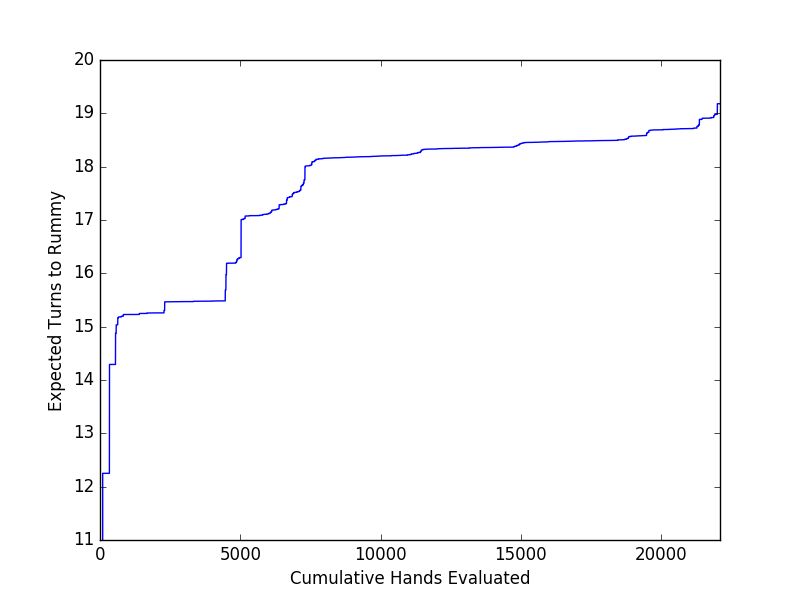
\includegraphics[width=\textwidth]{fig1.png}
\caption{Summary of E for 3-Card Aces Low}\label{fig:1}
\end{figure}

We can make some qualitative observations based on this graph. The expected time increases rapidly for the first few iterations, then levels off with values slightly greater than 15 for more than 4,000 hands. We might think of these as ‘good’ hands, while all the ones that come after might be thought of as ‘bad’ hands. Such subjective simplifications are mere heuristics for now, but they may come in handy as we seek ways to simplify our understanding of larger and more complex games. 

\subsubsection{Analysis of Results for 3-Card Rummy with Aces High or Low}

In the future, we will concentrate mostly on Aces Low rules since they are the most natural of the Ace conditions. However, the relative invariance of the results under Ace High rules is somewhat interesting. In increasing the flexibility of the Ace, Two, King, and Queen cards, the Ace High rules somewhat reduce $E$ values overall. By the end of the calculation the accumulated change results in this smaller lower bound:

$$\texttt{12 hands like A$\clubsuit$ 2$\diamondsuit$ K$\diamondsuit$ with E = 18.861678332 (22100 total)}$$

Those hands which consist of A2K of three different suits immediately precede this group, but with an E that differs in the hundredths place. When many equivalence classes are separated by orders of magnitude less, the difference is clearly significant. The reason for this distinction is not intuitively obvious, but it is proven true nonetheless. 

\subsubsection{Analysis of Results for 3-Card Continuity Rummy}

Continuity, or Round-the-Corner Rummy, vastly expands the symmetries that govern our equivalence groups. Since each card value can be incorporated into a full three runs, there are no least-useful cards like the aces and kings were before. This removes the end effects that we used to intuit the worst hands for other rule sets, and reduces the qualities governing a hand’s goodness or badness to the relative, rather than absolute, positions of the cards it contains, and the relative homo- or heterogeneity of their suits. With symmetry over the suits and the values, the minimum size of an equivalence class is now 52 hands. The largest equivalence class balloons up to: 

$$\texttt{1768 hands like A$\clubsuit$ 2$\clubsuit$ 3$\diamondsuit$ with E= 15.228977272 (2912 total)}$$

Unlike before, it is the set of hands solved by not the 12th but the 4th iteration of the dynamic program. The overall scheme of equivalence classes is even more compressed: there are only 60 of them (as enumerated in Appendix 2). The median equivalence class consists of 312 hands rather than 24 (though it is worth noting that these numbers do have something in common, as each is six times the smallest possible class). The form of our highest-E hands is difficult to intuit, and quite different from what came before: 

$$\texttt{52 hands like A$\clubsuit$  4$\clubsuit$  7$\clubsuit$  with E= 18.24424854000194 (22100 total)}$$

With such radical changes from our other two rule sets apparent in these metrics, we might question whether the overall contour of the accumulation curve will be radically different as well. The answer is: not quite. As seen in Figure \ref{fig:2}, the curve for this wrap-around rule set is chunkier, lower, and slower than the curves for the other two rule sets, but it follows a similar path overall. There is still the same sudden jump from ‘good’ hands to ‘bad’, though this one occurs more than 6,000 hands deep rather than 5,000 hands. This jump is also more precipitous: there are  actually no hands whatsoever whose $E$ begin with 16 under Continuity rules (one class has $E \approx 15.98$, the next has $E \approx 17.01$). But as we can see on the graph, it is qualitatively speaking a very similar jump. 

\begin{figure}
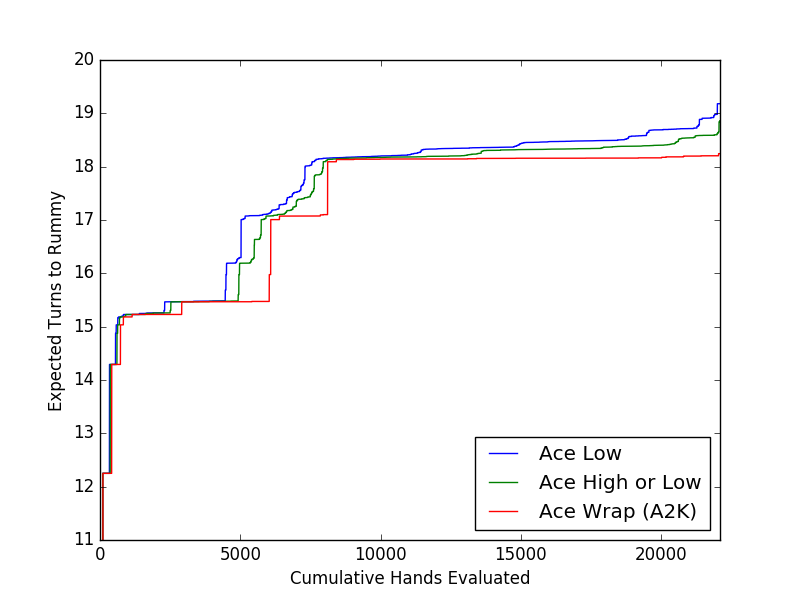
\includegraphics[width=\textwidth]{fig2.png}
\caption{Summary of E for 3-Card Rummy with Various Rules}\label{fig:2}
\end{figure}

What can we learn from this surprising similarity? It is apparent that the most important factor in the value of E for most hands is the relative position and suit of the cards to each other, with absolute end effects only interfering partially with these more powerful forces.  This near-congruence bodes well for our future efforts to simplify larger Rummy games. The Continuity Rummy’s dynamic program took only a half hour to run, a tiny fraction of the time required for the other two rule sets. If the most influential factor on policy ought to be the relative values and suits of cards, the construction of our policy function may be simplified immensely.

It is here that we pause and note that the output of our program, in aggregate, forms the basis for the hugely complex discrete policy function for these three rule sets describing games of 3-card rummy. It serves as a dictionary for evaluating $\min_{a\in \Gamma_x(h)}\{T_x(h,a)\}$ in all situations, thus finding what is expected to be the objective best move. While it will not guarantee a win in all situations, this counts as optimal play; for any hand $h_0$, E will be reduced from $E(h_0)$ to 0 as quickly as possible under the circumstances. 3-card Rummy is solved. 

\section{Four-Card Rummy}

\subsection{Combinatorial Regrowth}

Compared to the efficiency with which 3-card Rummy could be handled, 4-card Rummy sees a rise in complexity. The formula for the number of calculations which must be conducted remains the same, but with the size of $H$ having grown to $\binom{52}{4} = 270,725$, a typical iteration early in the process will now require 12 times as many calculations simply because there are 12 times as many hands. Likewise, because of the radically increased number of potential symmetries, the total number of iterations required will be several times larger than for 3-card Rummy. The computational times required become much higher, stretching to the dozens of hours compared to 3-card's dozens of minutes.

There are fewer Rummies in the 4-card game, as well. This is due to the lost flexibility of the sets. Whereas each card value produced four potential sets in 3-card Rummy, to get a 4-card set requires four-of-a-kind. As a result, there are only $4*10 + 13 = 53$ Rummies to start with, and fewer opportunities for 'adjacency' - the best hands in any rule set are those which are adjacent to two Rummies, not four, resulting in a first generation $E$ of $\frac{52-4}{2} = 24$ turns.

\subsection{Analysis of Results for 4-Card Continuity Rummy}

Due to the high symmetry of Continuity Rummy, it was possible to run the calculation at full precision in a reasonable time frame. We find that there are 2496 'best' hands with $E=24$ as mentioned above, slightly less than 1$\%$ of the total. The worst hands are these:

$$\texttt{156 hands like A$\clubsuit$ 2$\diamondsuit$ 5$\clubsuit$ 6$\diamondsuit$ with E = 38.6563243418}$$

Figure \ref{fig:3} illustrates the complete summary of the results. The strictures of 4-Card Rummy are unforgiving. Games would be expected to last much, much longer than 3-Card rummy because it is much more difficult to arrange all four required cards. This indicates that in the games of 7-card and 10-card Rummy, it would be the acquisition of a 4-card meld which would be the bottleneck.

\begin{figure}
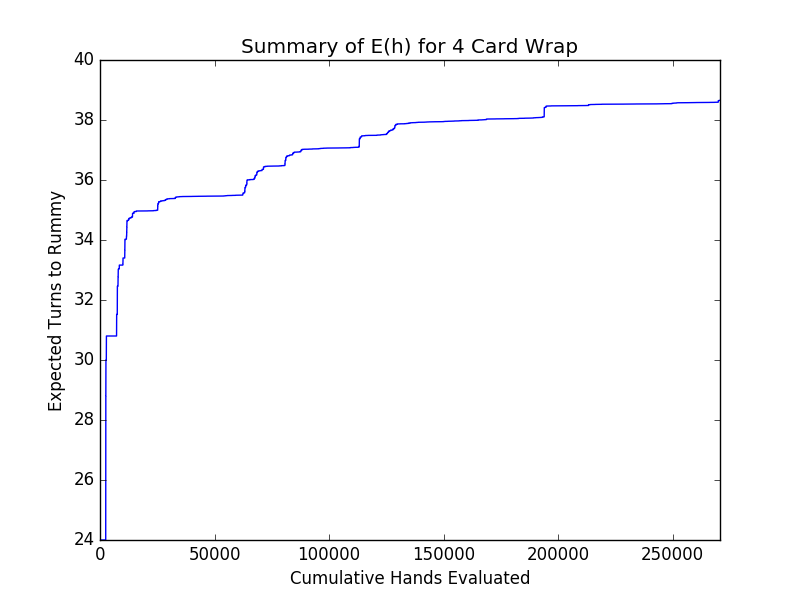
\includegraphics[width=\textwidth]{fig3.png}
\caption{4-card Wrap}\label{fig:3}
\end{figure}

The resulting output featured 654 equivalence classes as compared to 3-Card Continuity's mere 60. The ratio $\frac{654}{60} \approx \frac{270725}{22100}$, indicating that the number of equivalence classes may grow roughly in proportion with the number of hands. We may conjecture that 7-card Continuity Rummy would have roughly $\frac{\binom{52}{7}}{270725} * 654 \approx 300,000$ such classes - a dispiriting estimate to be sure. Our approach, while the most rigorous available, may not be readily applicable to games larger than 4-card Rummy. In fact, even 4-Card Rummy with Aces low invites difficulties of scale, as we may conjecture that it will require a similarly greater number of equivalence classes to fully describe. For 3-Card Rummy the ratio from Wrap to Aces Low was 60:688. If the results for 4-Card are similar we will have $\frac{654}{60} * 688 \approx 7000$ classes on our hands - hardly a summary at all.

While our interest began with optimization, it has become clear that the scale of the problem is such that finding the true optimal solution may not always be efficient, and that the marginal utility of such aggressive optimization may not be worth the computational effort. Let us now consider methods for finding satisficing strategies - those which are good, but not necessarily perfect.

\section{Approximation and Least Upper Bounds}

\subsection{An Illustration of the Bounding Process}

Consider a hand $h$ of 3 non-adjacent cards arranged to have the minimum possible number of potentially-adjacent drawable cards. Under Ace-Low rules, this would be a hand containing an Ace, a King, and some other card between 4 and Jack. For the sake of illustration, let us declare that these cards are A$\clubsuit$, 7$\diamondsuit$, K$\heartsuit$. For such hand, each of the three cards presents three other options which could result in a pair of the same value, and there are also two cards which could result in a dual-ended two-card run (these being 6$\diamondsuit$ and 8$\diamondsuit$). Once one of these proto-sets or -runs is established, there are two remaining cards which could complete it.

In order to place an upper bound on $E$ for all hands in $H$, we may use the expected value results achieved in Theorem 1.2 to determine how long it will take to produce a hand with a valid pair, and then once a pair is established how long it will take to complete it. Because there are a total of 11 cards which will give us a pair, we expect it to take $\frac{49}{11}$ turns to create a pair. Once a pair is achieved, we expect it to take $\frac{49}{2}$ turns to complete it. As such, we expect that an upper bound for all hands in 3-card Rummy is around 29 turns.

As it turns out, this is a very bad upper bound. The true least upper bound, as mentioned in section 3.1.1, is around 19.18. But the general strategy here is sound - if we establish how long it takes to get to a known class of better hand, we can derive an upper bound from the time it takes to reach to that class of hand and that class' own $E$. In essence, we are generating an approximation by choosing a strategy which is willfully obtuse, intentionally ignoring potential improvements in exchange for increased simplicity.

How can we refine the strategy? Well, for starters, we need not rely on getting to just one class of hand. For the hand above there are two cards which lead to two-card runs which are single-ended (these being 2$\clubsuit$ and Q$\heartsuit$). Because we are playing with aces low rules, these each have only one card which can complete them, which gives them an $E$ of 49 in our naive current scheme. But how are we to integrate this with the other cards that have different, better future values for $E$? As it happens, we already have a tool for such calculation: the Bellman Sum.

\subsection{Implementation of the Approximation Algorithm}

Recall that the general strategy for calculating $E$ was to, for each iteration, calculate the quantity $E_{hyp}$ for each $h$ in $H'$, then 'lock in' the value of $E$ for each $h$ whose $E_{hyp}$ was equivalent to the global minimum of the current set of $\{E_{hyp}(h) | h \in H' \}$. When this process was automated, however, allowances had to be made for the non-arbitrary precision of computer arithmetic. Due to floating-point errors in the evaluation of the Bellman Sum, hands which are in fact symmetrical might end up with values for $E$ which differ slightly beyond the eight decimal place. In order to fix this problem, the program featured a check not for equality, but for proximity within a certain tolerance.  Here is an example from $\texttt{3cardRummyLow.cpp}$ (where $\texttt{minE}$ is the minimum $E_{hyp}$ for the current iteration:

\begin{verbatim}
for(int i=0; i<22100; i++){
    if(hands[i]->getE()-minE < 0.0000001 && !hands[i]->getLockedIn()){
        hands[i]->lockIn();
        locked++;
        //output procedure omitted
    }
}
\end{verbatim}
The tolerance was hardcoded as $10^{-8}$ during the initial implementation to ensure eight digits of significance in the results. But if all we seek is an approximation, an upper bound, then the tolerance can be increased to some arbitrary value like so:

\begin{verbatim}
double tol = 0.1; //for example

for(int i=0; i<22100; i++){
    if(hands[i]->getE()-minE < tol && !hands[i]->getLockedIn()){
        hands[i]->lockIn();
        locked++;
        //output procedure omitted
    }
}
\end{verbatim}

On each generation, this will in effect decide that a hand's current $E_{hyp}$ is 'good enough' if it is within the tolerance range of the current minimum $E_{hyp}$ and finalize it prematurely. Then, using the prematurely finalized values it will go on to calculate the next iteration's $E_{hyp}$ and so on. This technique is only useful if the error does not cascade with each successive calculation. Fortunately we can bound the error for this process as $t$ = tolerance all the way through to the end.

\begin{theorem}
For a given tolerance $t$, the maximum error generated by the Bellman Sum algorithm for calculating expected time to Rummy will be bounded by $t$.
\end{theorem}

\begin{proof}
We will prove by induction. For the base case, consider the first iteration of the procedure. Those hands closest to Rummy will have their true $E$ calculated and that $E$ will be the first $E_{min} = \min_{h \in H'} \{E_{hyp}(h)\}$. Now consider some other hand $h_0$ which will be locked in. It will have $E_{hyp}(h_0) < E_{min} + t$. Because the development of a given hand's $E_{hyp}$ is monotonic over the course of the iterations, the true value $E(h_0)$ must be less than $E_{hyp}(h_0)$. So we have $E_{min} < E(h_0) < E_{hyp}(h_0) < E_{min} + t \implies E_{hyp}(h_0) - E(h_0) < t$, as desired.

Now, suppose we have an iteration where $\forall h \notin H'$ there is a known satisficing approximation $E^*(h) \ni E^*(h) - E(h) < t$. Note that regardless of the tolerance used to perform the calculation, it will still be the case that $\max_{h \in H\setminus H'}\{E^*(h)\} < \min_{h \in H'}\{E_{hyp}^*(h)\}$ at each iteration (i.e., no worse hand may sneak into the set of finalized hands before a better hand). Because this is the case, there will be some subset of $H'$ for which every element of $X'$ has an associated $E^*(T_x(h_0,a))$. For members of this subset, we will have

$$E_{hyp}^*(h_0) = \frac{49+\sum_{x\in X'} E^*(T_x(h_0,a))}{|X'|} <  \frac{49+\sum_{x\in X'} (E(T_x(h_0,a))+t)}{|X'|} = $$

$$\frac{49+\sum_{x\in X'} E(T_x(h_0,a))+|X'| \cdot t}{|X'|} = E(h_0) + t$$

Indeed, for each $x \in X$ we may introduce an error of up to $t$ to the term $E(T_x(h,a))$ and still retrieve a result for $E_{hyp}^*(h)$ which is within $t$ of $E(h)$.

Consider those members of $H'$ for which not all of the cards that should be in a proper $X'$ have associated future hands that are yet finalized. Let us say that for a hand $h_1$ there is at least one future hand $T_x(h_1,a_m) = h_m$. What is the nature of these missing future hands? By definition they are better than $h_1$. This means that they are also among those hands for which $E_{hyp}^*(h_m) < \min_{h \in H'}\{E_{hyp}^*(h)\}+t$, i.e. those hands which are set to be locked in during the current iteration. This implies that $E_{hyp}^*(h_1)-E_{hyp}^*(h_m) < t$. Due to the monotonicity of the progression of $E_{hyp}$ for each hand this proximity will translate to their true values as well. The upshot is that for each of the future hands like $h_m$ which ought to add members to $X'$ but don't, we will not be introducing an error of more than $t$ by assuming instead that each $x$ generates the hand $h_1$. In so doing we may still solve the sum for $E_{hyp}^*(h_1)$ as before without introducing error of more than $t$ in total, as each individual term will have error smaller than $t$.

Since the error will not grow during any iteration, the proof is concluded.
\end{proof}

What is the practical use of this approximation scheme? Well, since the errors are bounded by a constant we may produce data which is quite good while speeding up the process immensely - since each iteration finalizes far more than one equivalence class worth of hands, the program will execute more rapidly. This alacrity allowed us to examine the effects of many different tolerances, from 1.0 to 0.001, on the calculation. Even if there are some aspects of the above outline which could use further rigor, the empirical evidence speaks for itself.
 
\subsection{Approximation of 3-Card Rummy with Aces Low}

In order to test the validity of this approximation scheme, it was applied to the already-solved problem of 3-Card Rummy. Even seemingly large tolerances result in surprisingly accurate results. Figure \ref{fig:4} shows the actual $E$ arranged in ascending order for Ace Low (the blue line) along with the approximations achieved by iterating with a tolerance of 1.0.

\begin{figure}
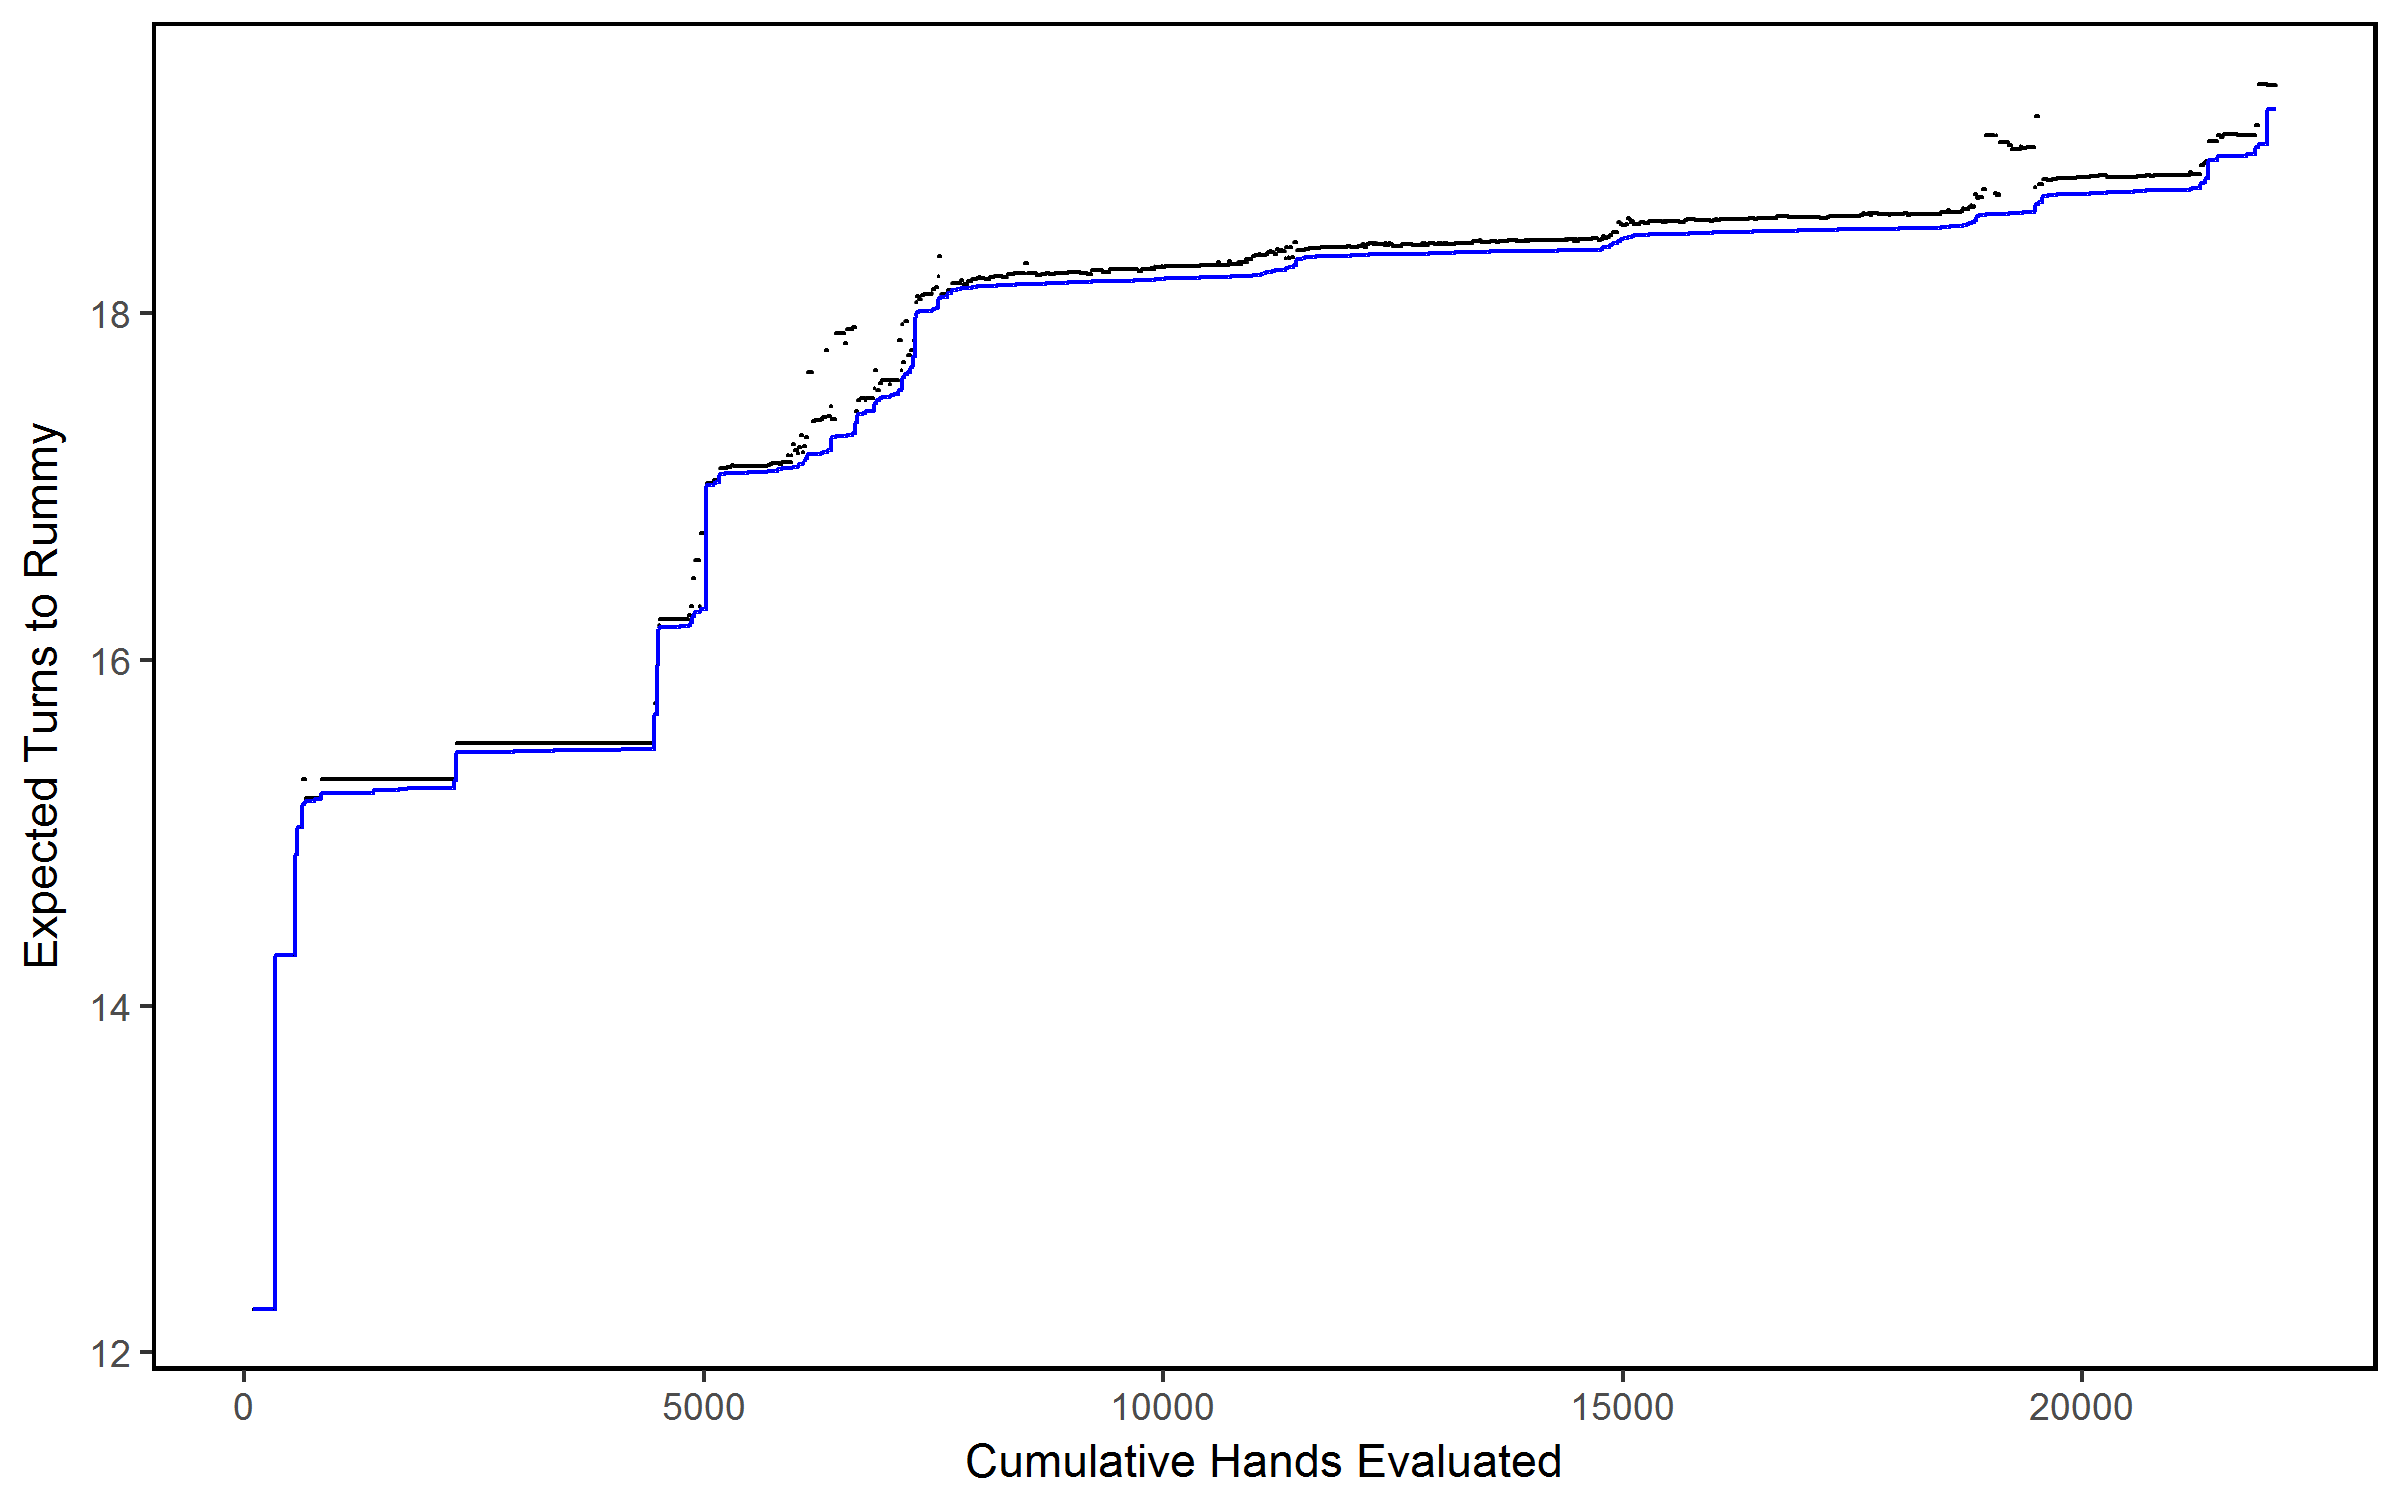
\includegraphics[width=\textwidth]{fig4.png}
\caption{3-Card Ace Low Approximation with Tolerance 1 vs. Actual}\label{fig:4}
\end{figure}

With smaller tolerances, the deviations become even more minute, to the extent that they can barely be seen on a full graph. Figure \ref{fig:5} plots the error for each hand instead with a tolerance of 0.5, and Figure \ref{fig:6} shows a few more. In every case tested, the maximum error is significantly less than the tolerance itself. For $t=1$ the greatest error was with hands like $3\clubsuit 5\clubsuit \textrm{K}\clubsuit$; their upper bound came out 0.6109 turns higher than their true $E$. It is not easy to form an intuition for why this type hand should be less accurate than all the others. With $t=1$ the hands had a mean error of only 0.086. When $t=0.1$ the mean error is 0.019. Finally, when $t=10^{-3}$, the maximum error is $2.35*10^{-4}$ and the mean is smaller still, $1.87 * 10^{-5}$. This consistent relationship, with tolerance greater than maximum greater than mean, is displayed for every tolerance tested - about a dozen in all. The empirical evidence is ample that our scheme works and produces predictably highly accurate results.

\begin{figure}
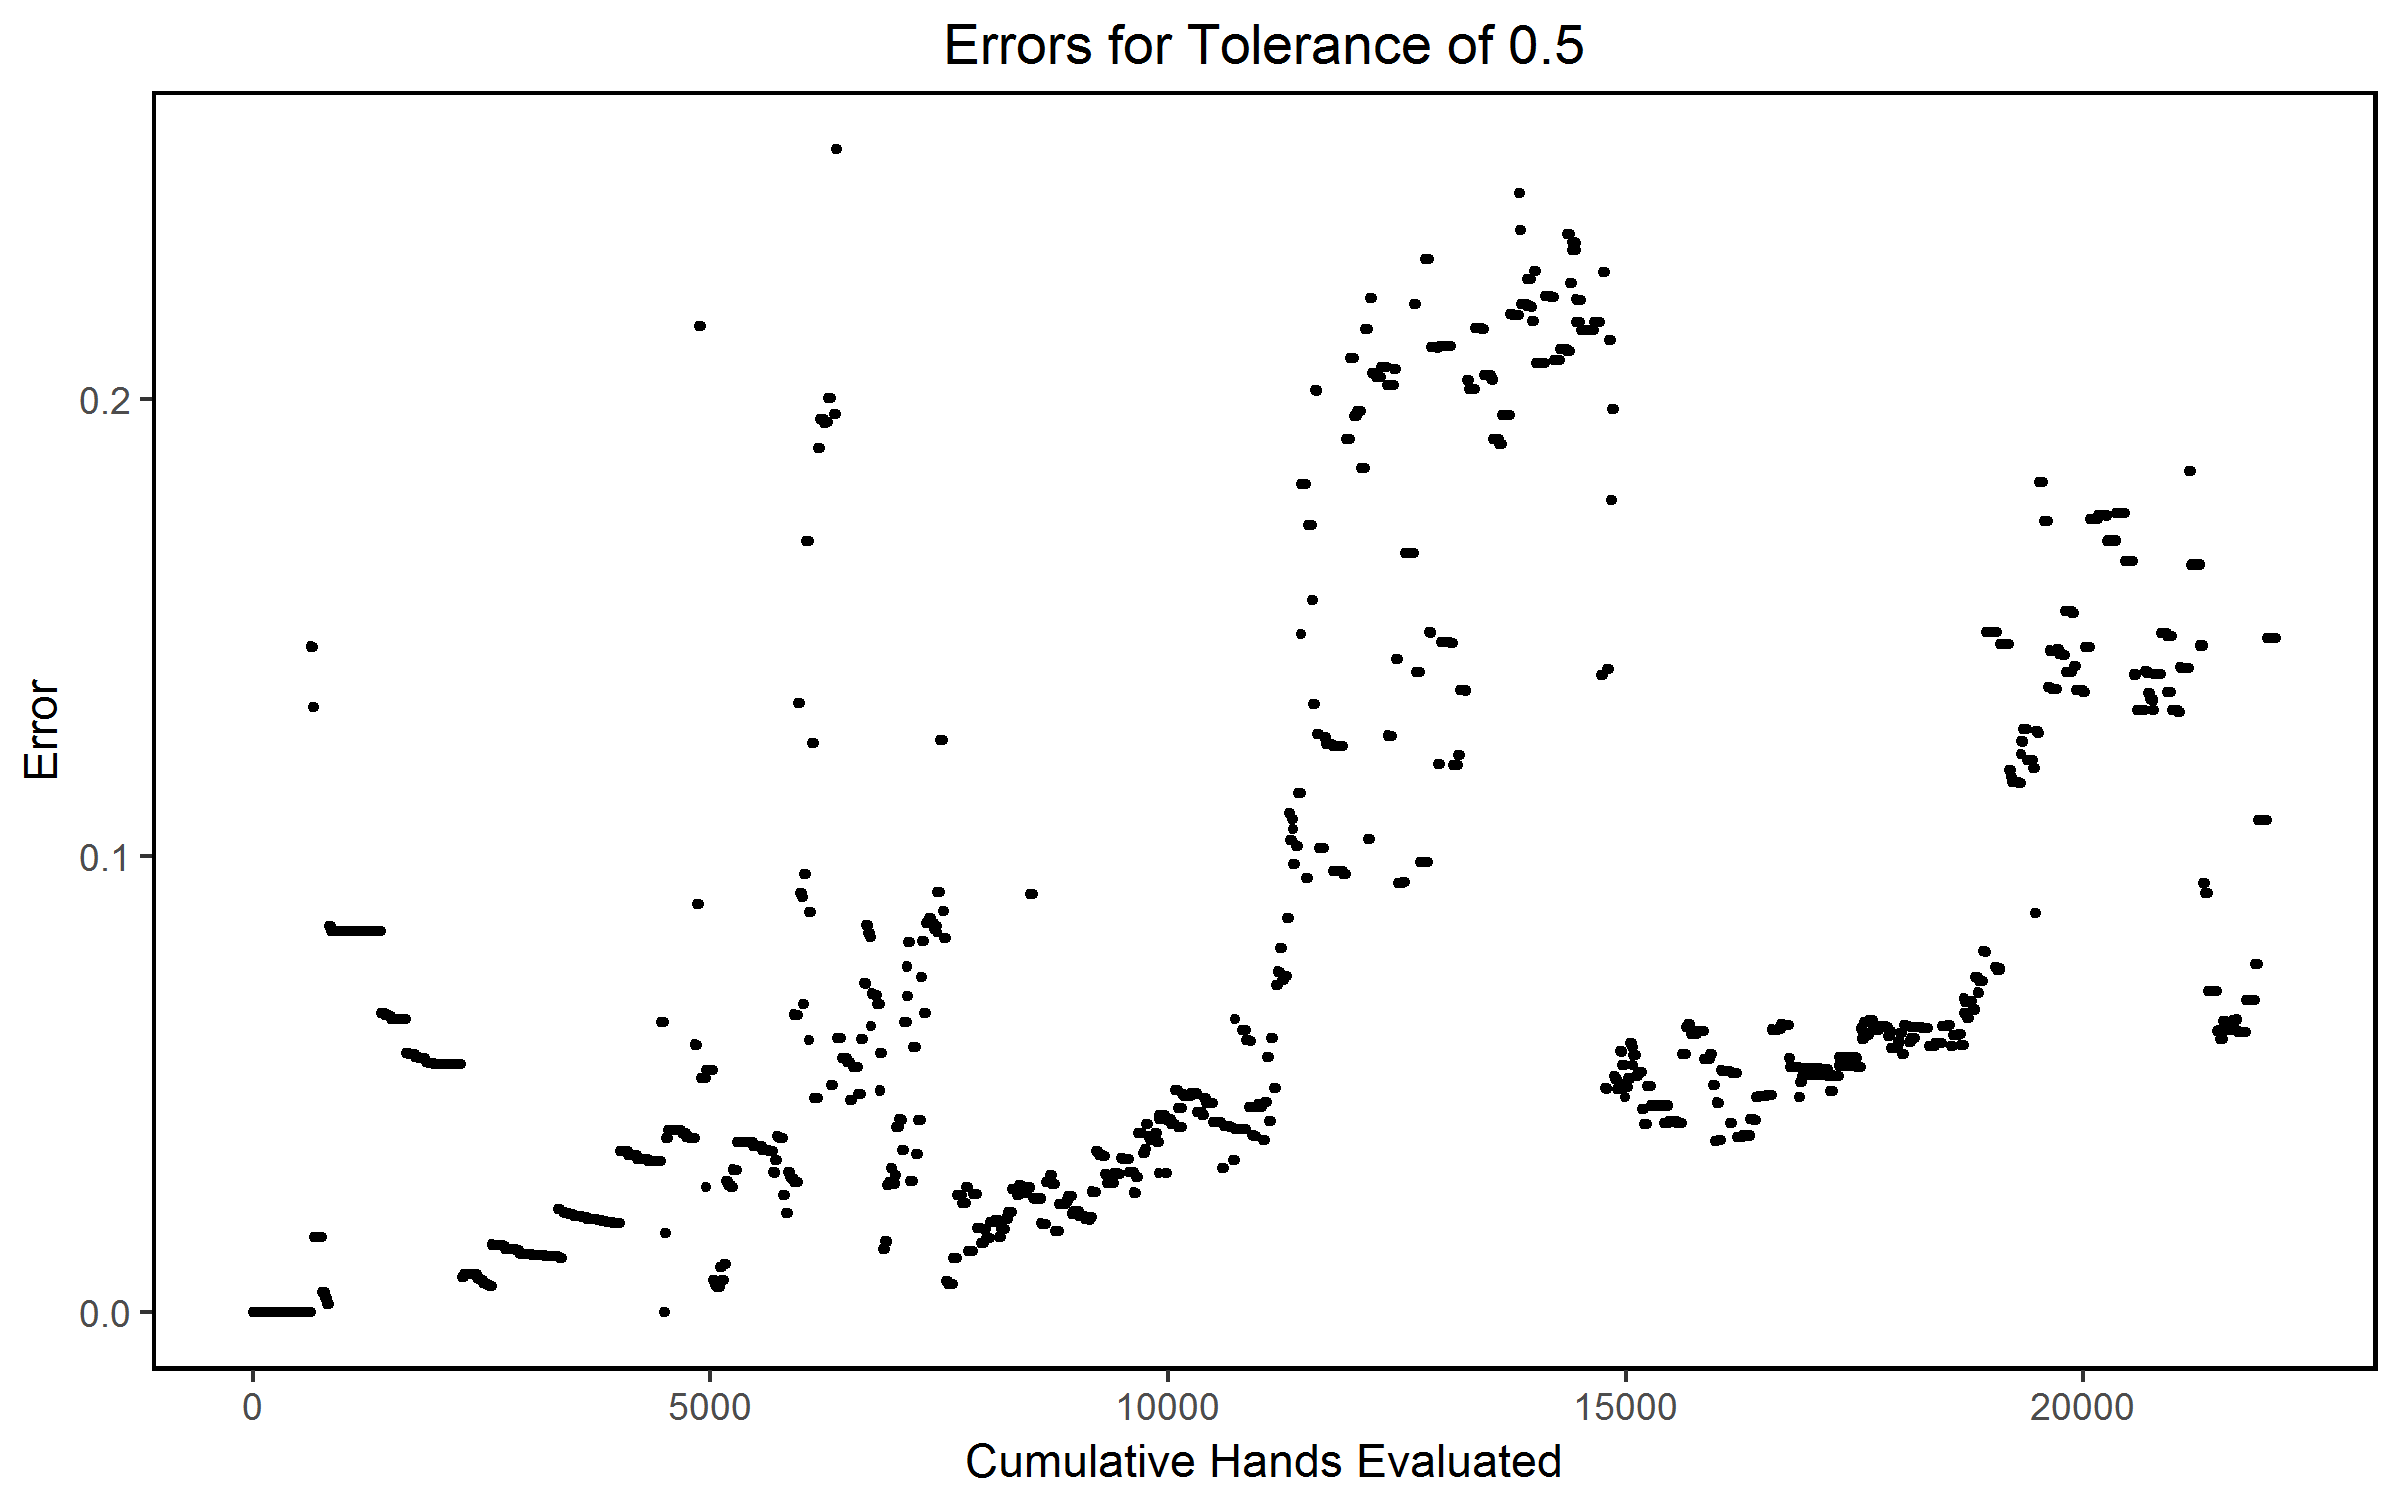
\includegraphics[width=\textwidth]{fig5.png}
\caption{Errors for Approximation with Tolerance of 0.5}\label{fig:5}
\end{figure}

\begin{figure}
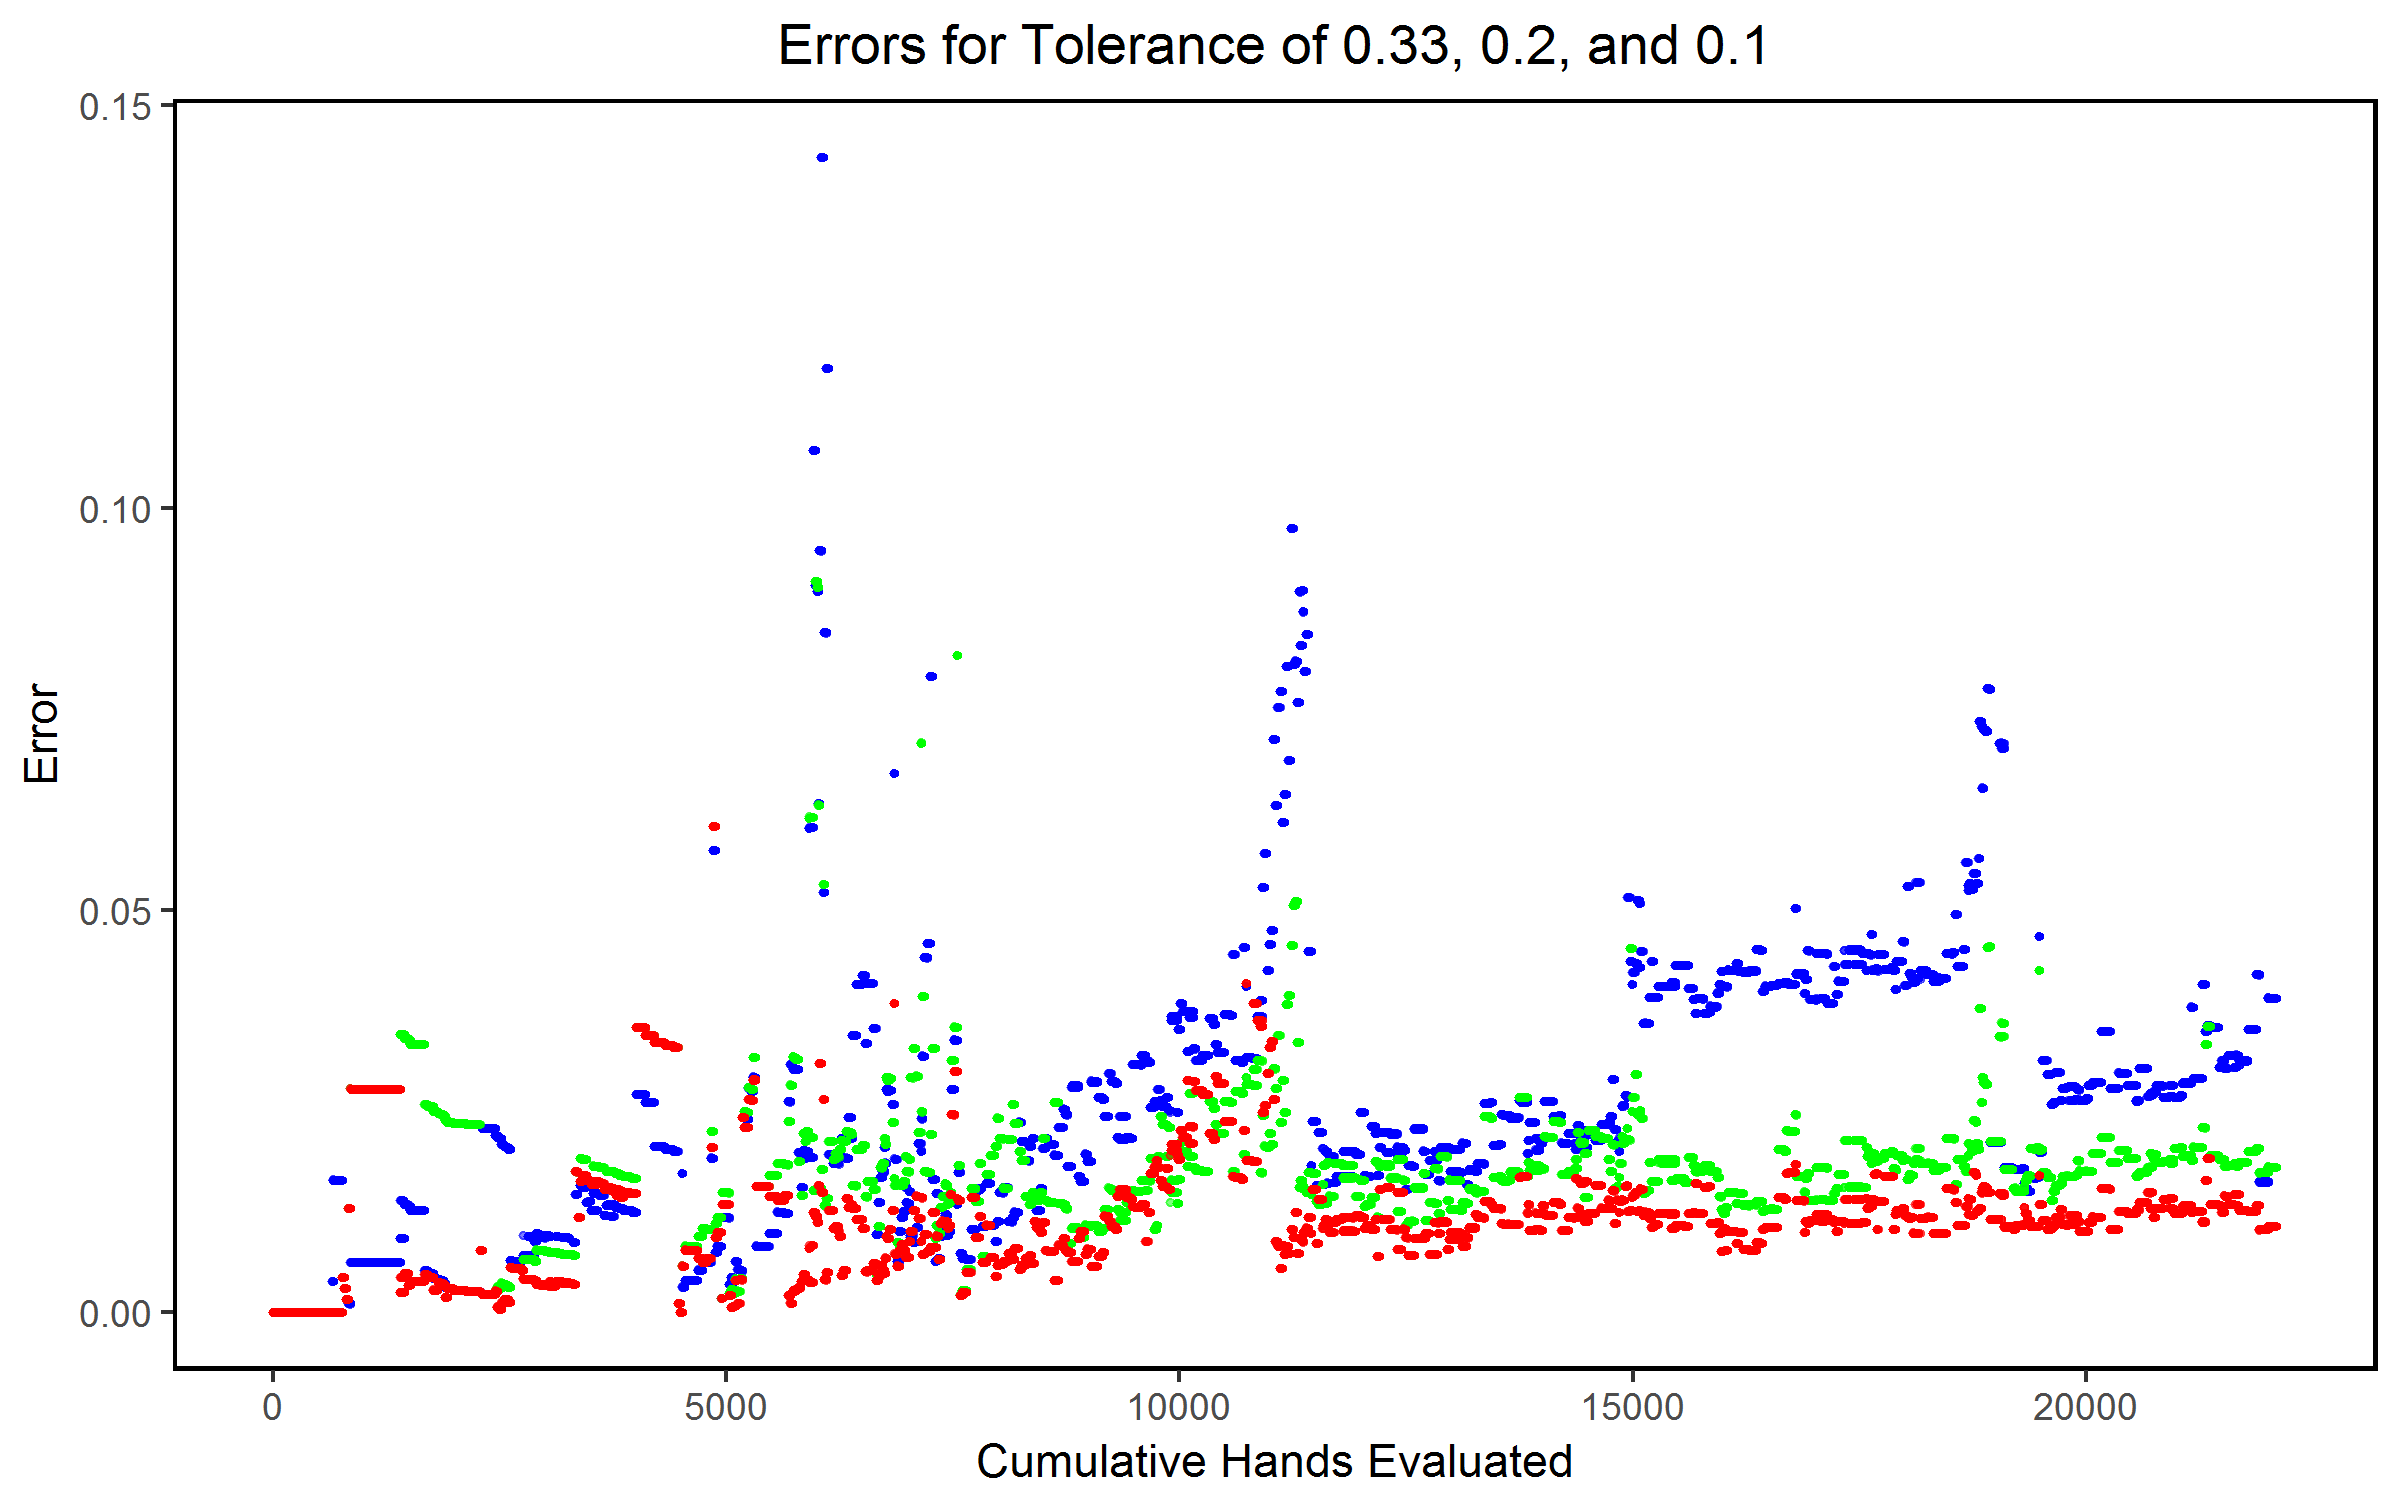
\includegraphics[width=\textwidth]{fig6.png}
\caption{Errors for Approximations with Tolerances of 0.33, 0.2, and 0.1}\label{fig:6}
\end{figure}


Since the motivation for this approximation was to increase the speed of our calculation, the next relevant question to pursue is the trade-off between accuracy and speed. Can we establish a relationship between tolerance and the time required to complete the calculation? In order to test this notion, we collected the duration of the calculation for 17 different $t$ values between 0.001 and 1. The results displayed a clear exponential nature. By performing a log transformation on the data we were able to obtain the following relationship via a standard linear regression:

$$time = \alpha * t^{-0.538}$$

where $\alpha$ is a proportionality constant depending upon the speed of the hardware. On the machine used to conduct the calculations, we had $\alpha = 7$. Figure \ref{fig:7} represents these data and the linear regression deduced from them.

\begin{figure}
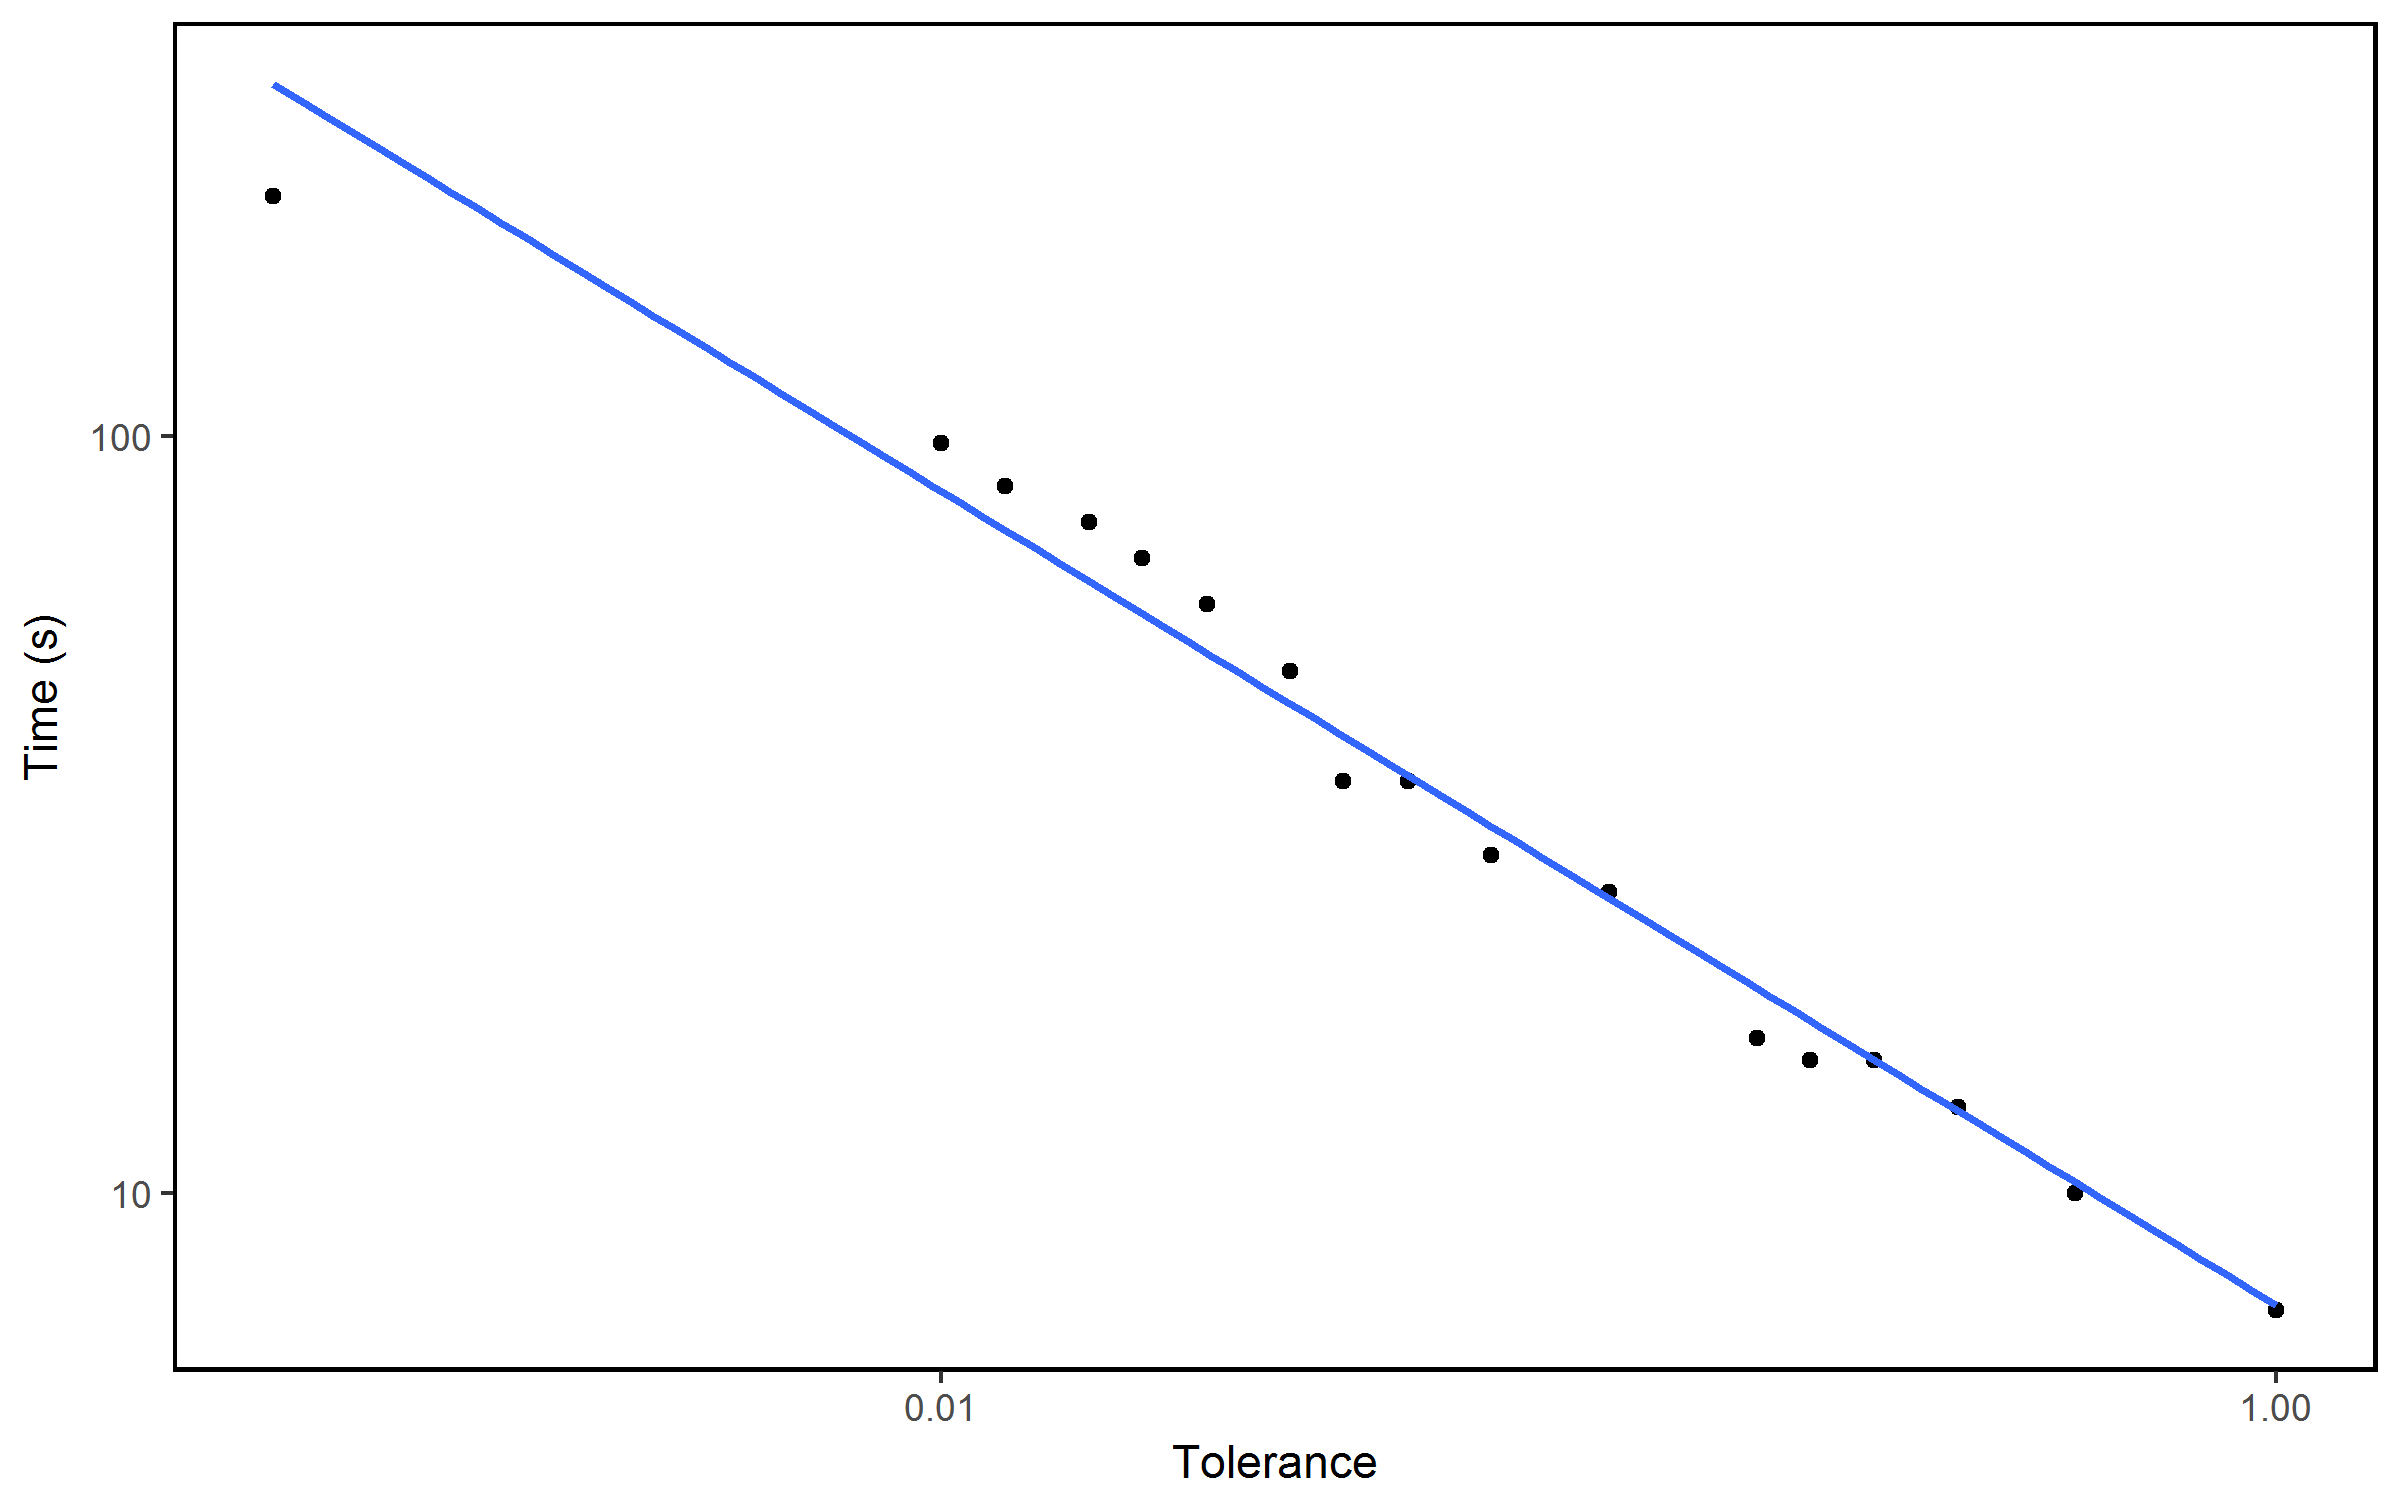
\includegraphics[width=\textwidth]{fig7.png}
\caption{Calculation Time vs. Tolerance (log scales) for 3-Card Approximation}\label{fig:7}
\end{figure}


We may use this relationship to estimate how long it will take to execute the calculation of 4-Card rummy for various tolerances, so that we can decide which are feasible and useful.

\subsection{Approximation of 4-Card Rummy with Aces Low}

To start off, let us perform the 4-Card approximation with a tolerance of 1, the largest viable value. The results are represented as points in Figure \ref{fig:8}.

\begin{figure}
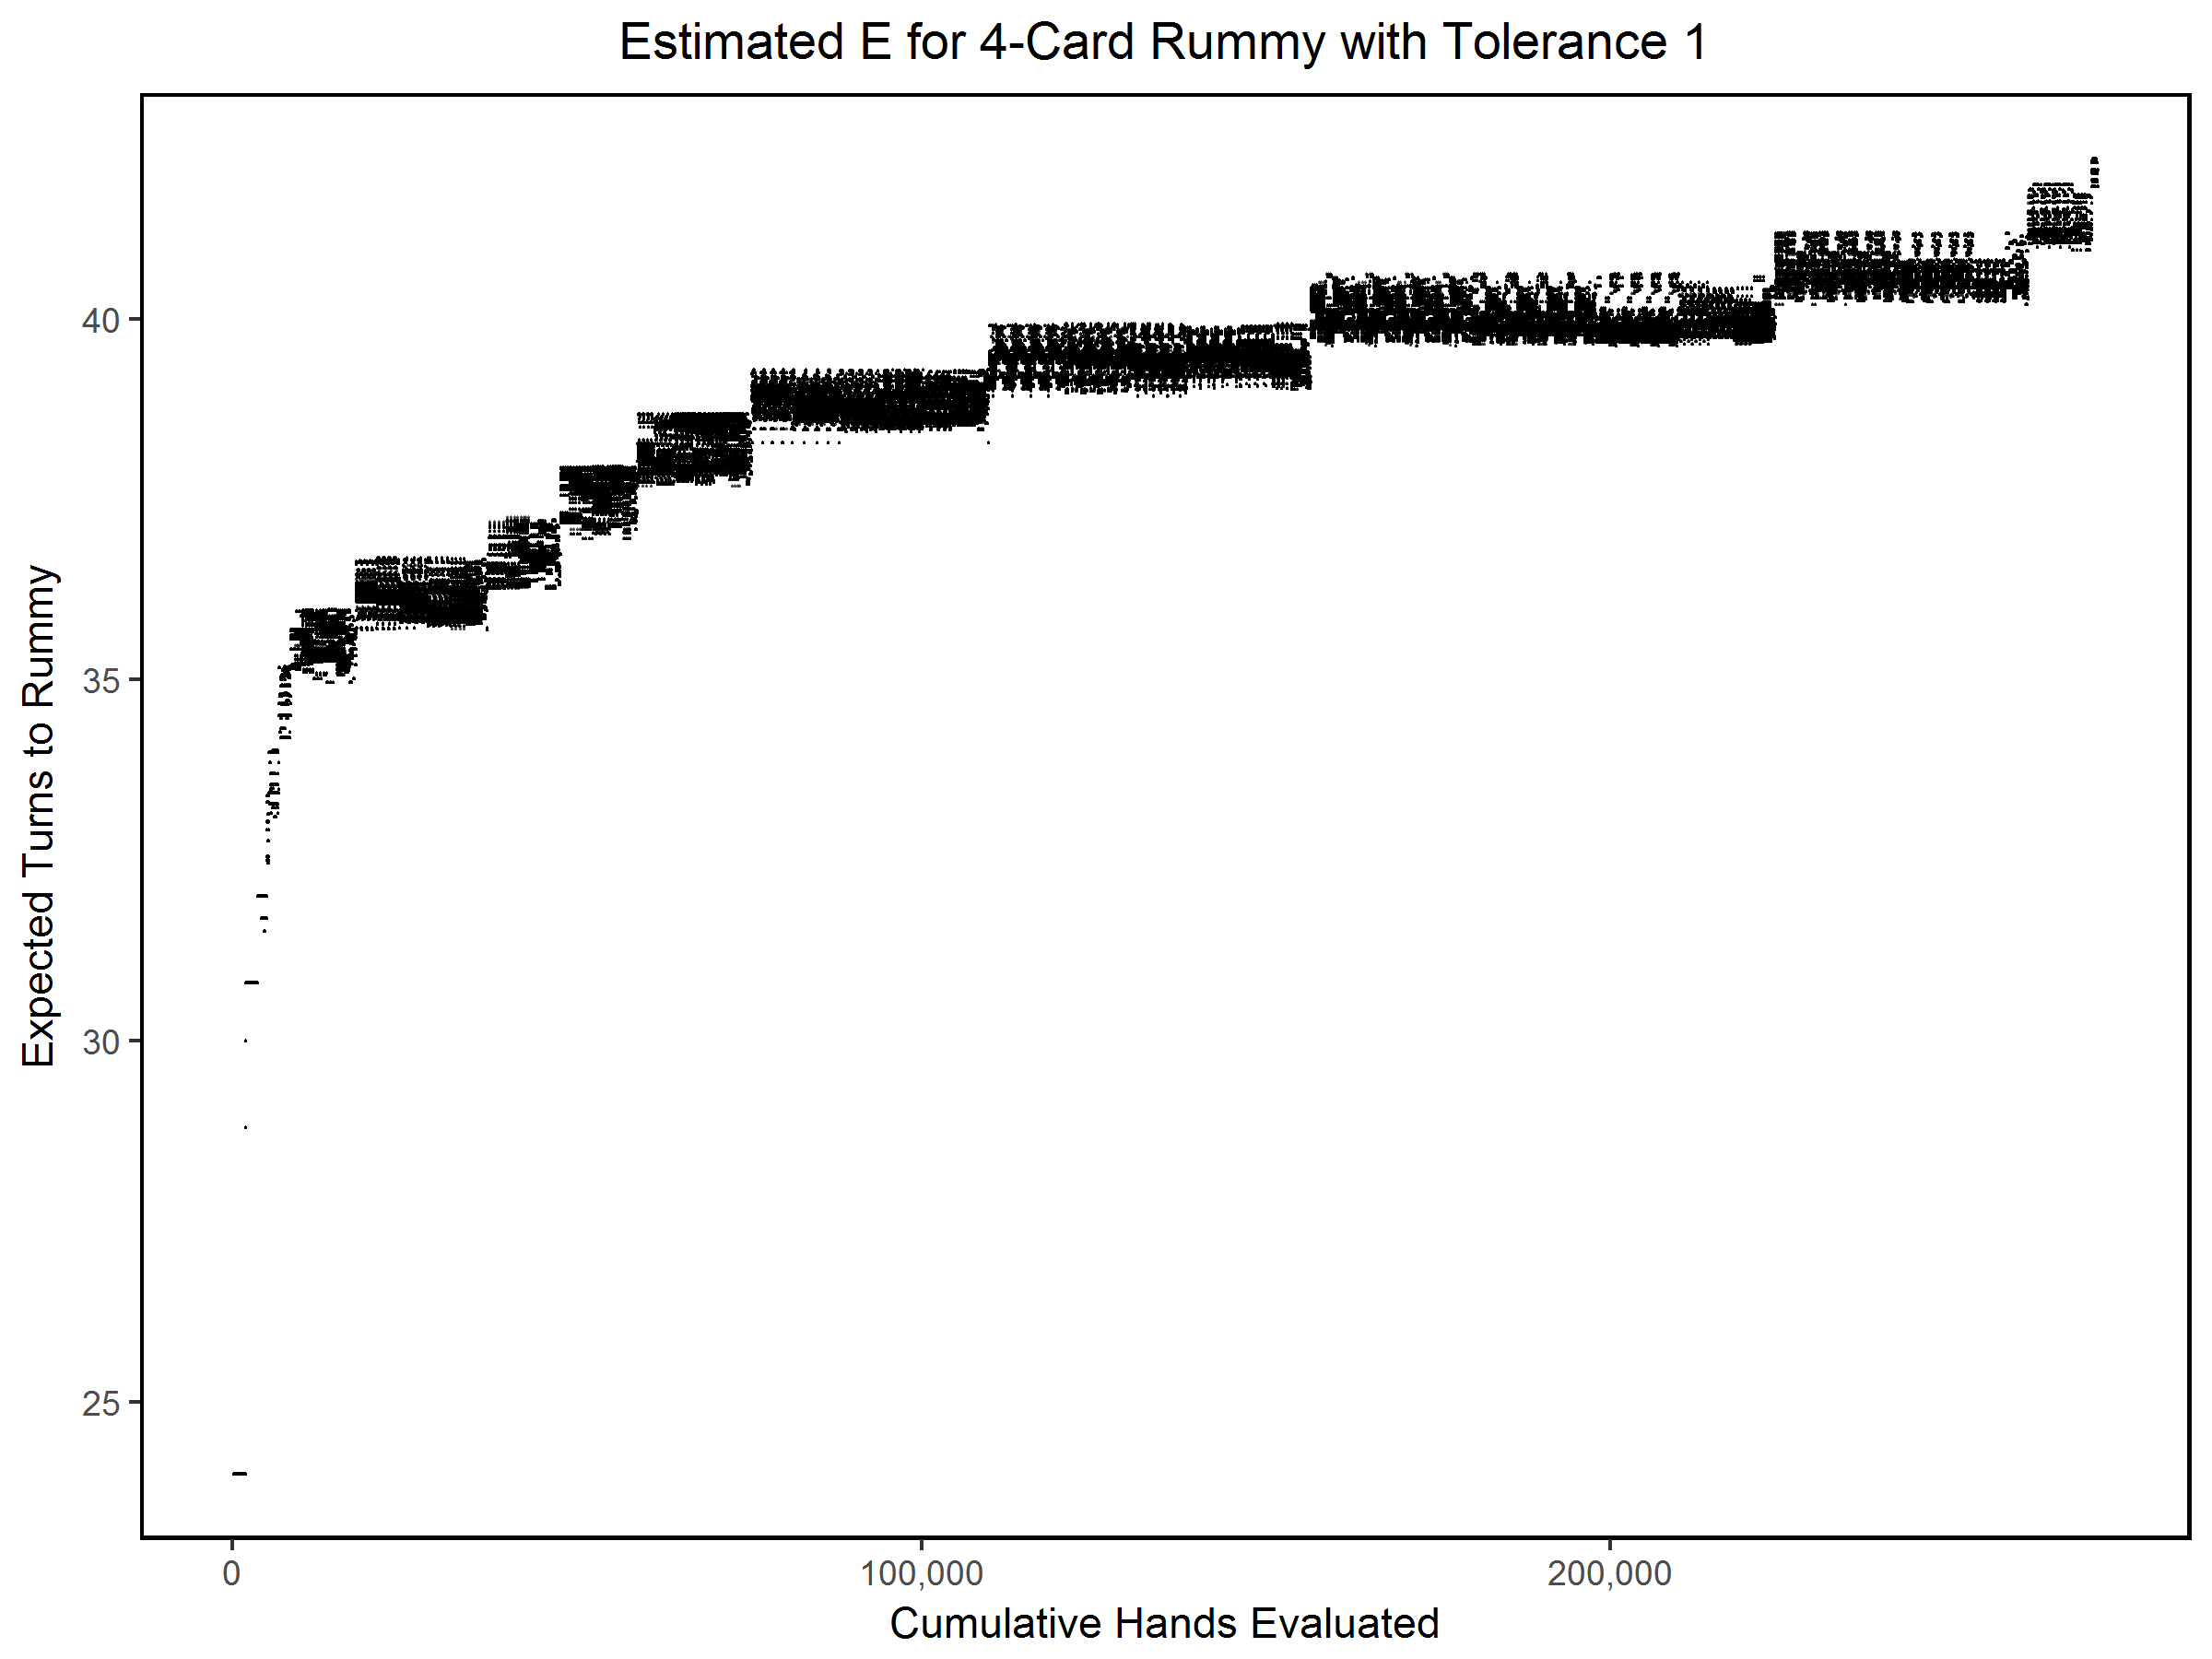
\includegraphics[width=\textwidth]{fig8.png}
\caption{Approximation of E for 4-card Rummy with Tolerance of 1}\label{fig:8}
\end{figure}


This approximation is much more riotous than the 3-Card data plotted in Figure \ref{fig:4}, with fuzzy clumps of values all along the apparent curve. The 270,672 non-Rummy hands were finalized in 19 cohorts, many of which can be seen qualitatively on the graph. (Compare this with the 7 cohorts of 3-Card Rummy with tolerance 1). The longest rectangle, fourth from the right, corresponds with the following program output:
$$\texttt{67468 hands like A$\clubsuit$ A$\diamondsuit$ 3$\clubsuit$ 3$\diamondsuit$ with E = 39.6312457202}$$

The program outputs as representative the minimum $E$ of the entire cohort, so for the 67,468 hands which were locked in on that iteration, $\min\{E_{hyp}^*\}$ was 39.6312457. 

This program ran in 225 seconds. Extrapolating from our model above, we would expect a tolerance of 0.001 to take at least $225 * 0.001^{-0.538} = 9250$ seconds. This seems feasible. First, however, let's try a few more large tolerances. Figure \ref{fig:9} shows the data in the order it was finalized for three more tolerances. We can see how it appears to converge towards a central curve. At this point a note on the appearance of the data is in order: When dealing with the 3-Card approximations, we could arrange the approximated data according to the correct ordering of the hands, since we already knew the true $E$ for each hand. Since we have not solved 4-Card rummy completely, such ordering cannot be achieved when displaying our approximations, resulting in the chaotic graphs, since within each cohort the points are arranged left-to-right in 'card order' (i.e. the order in which they were constructed by the triple loop), rather than in any coherent scheme.

\begin{figure}
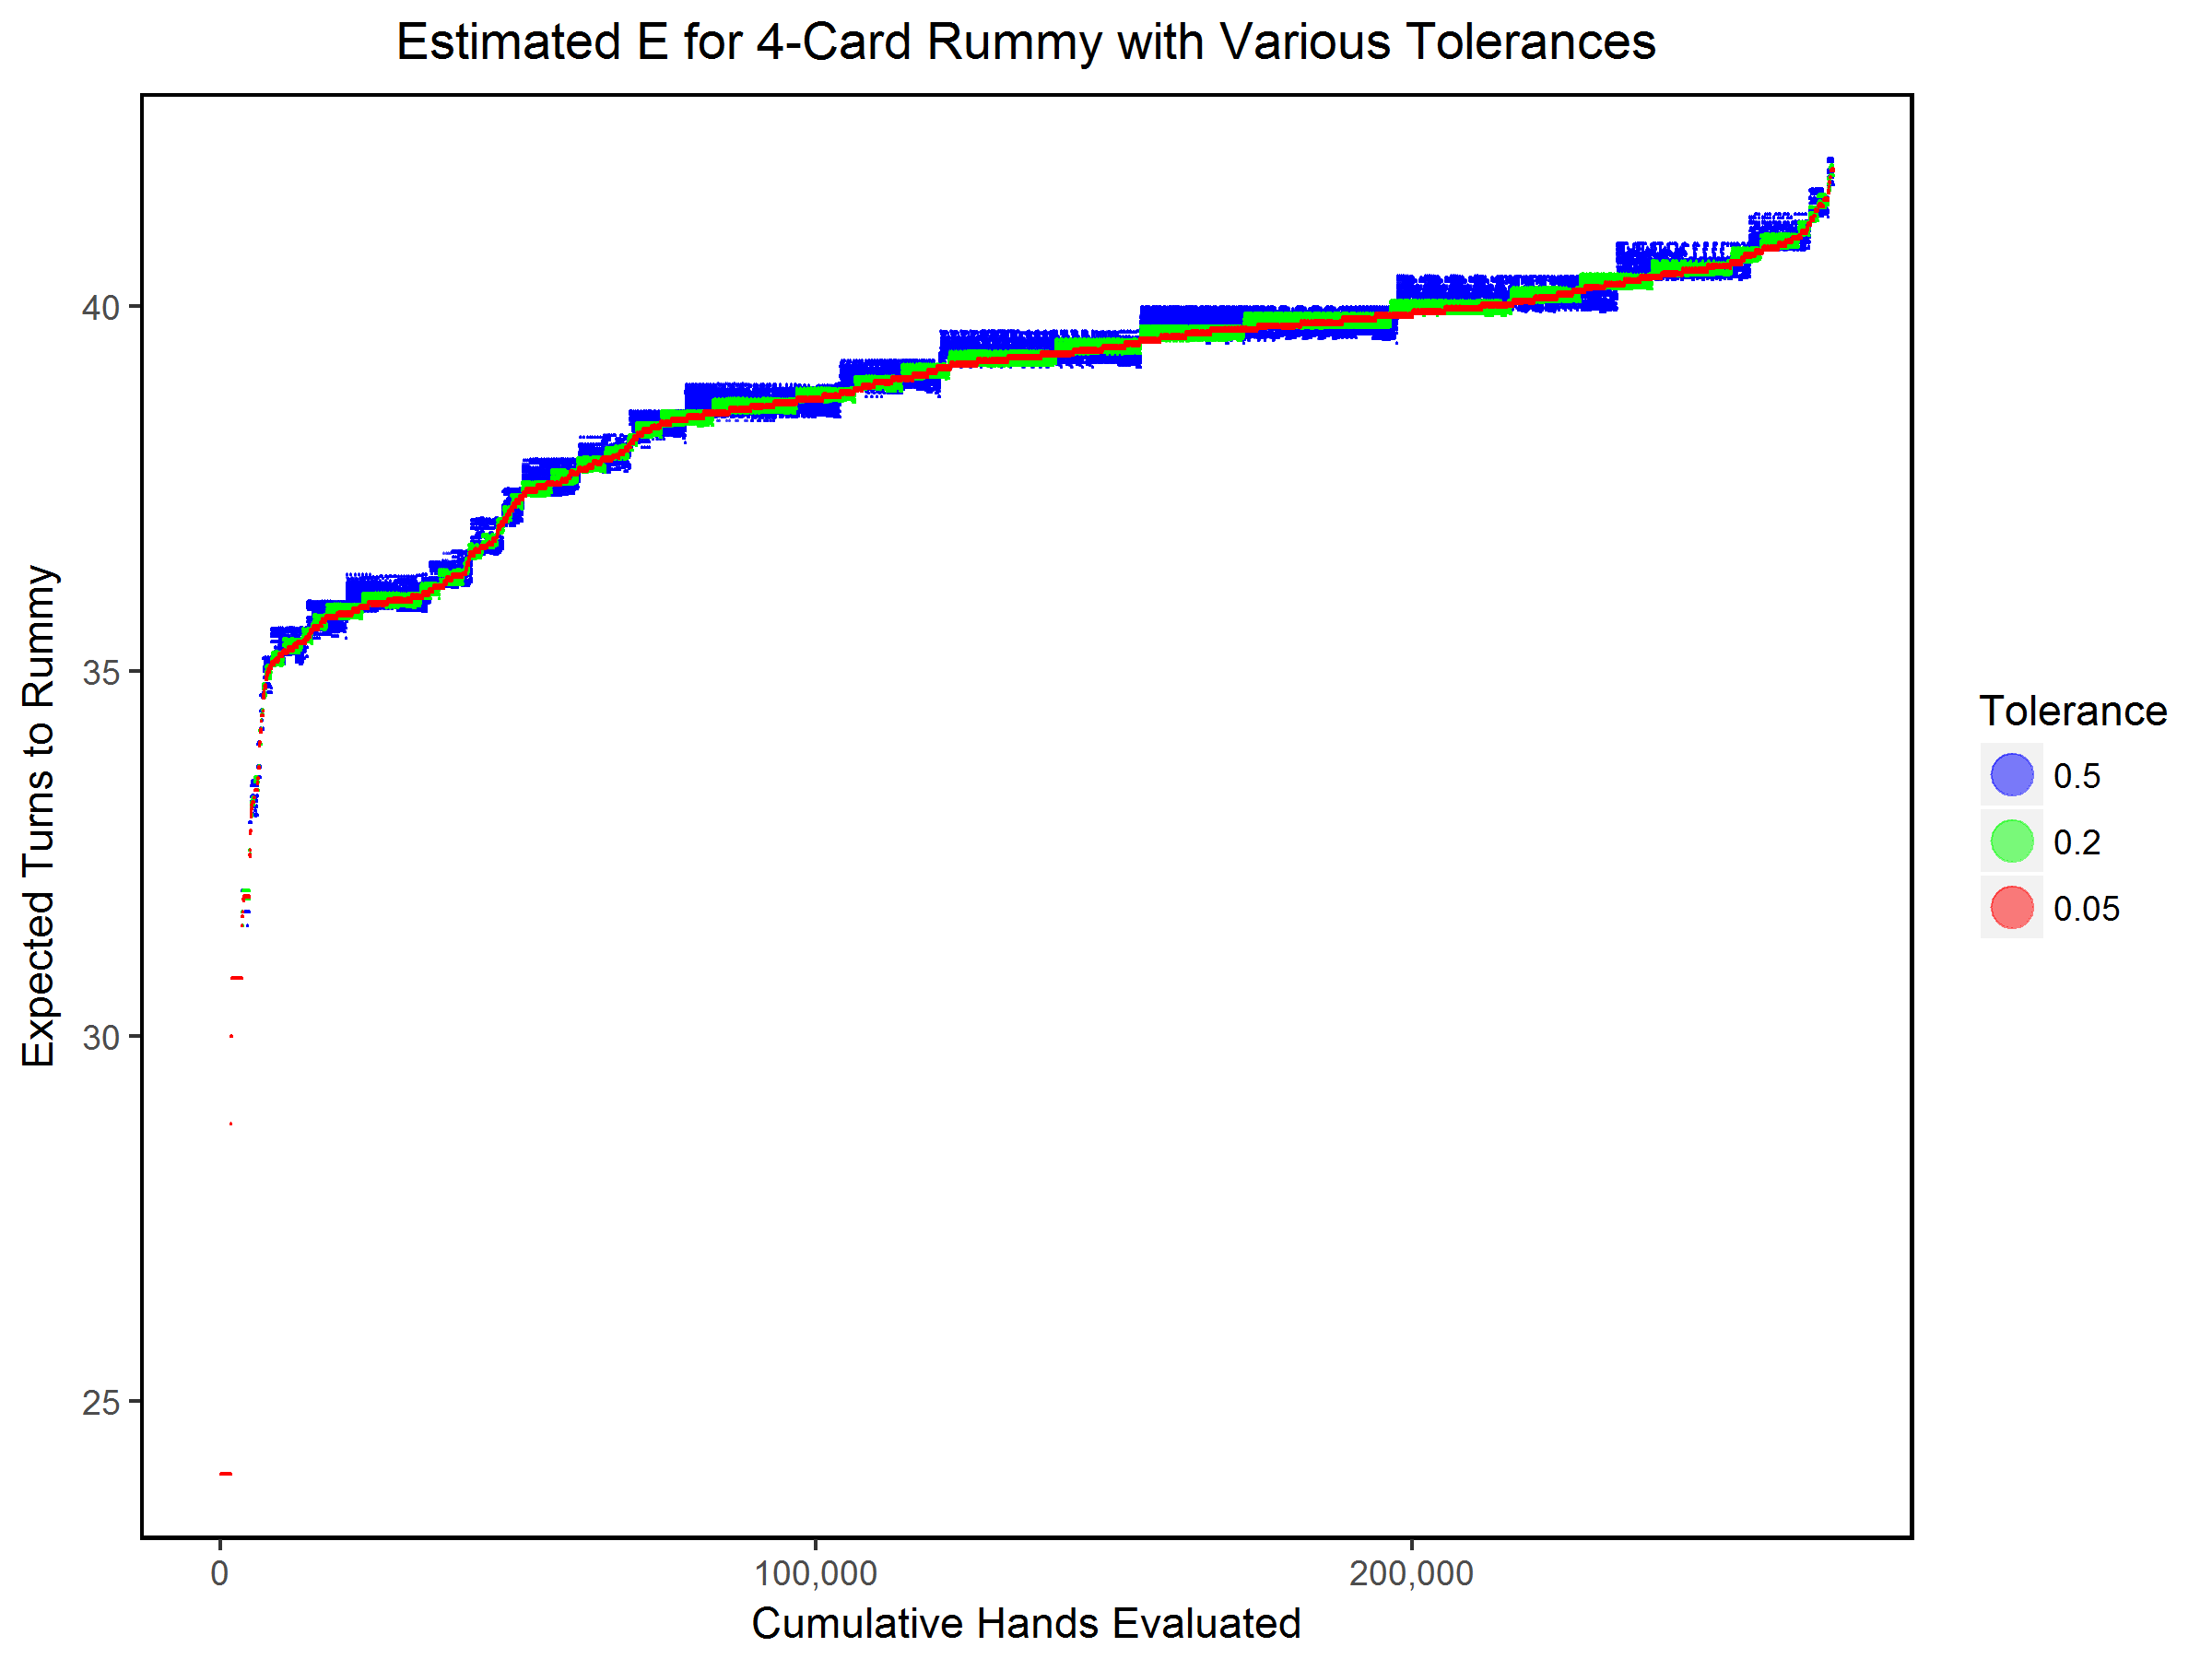
\includegraphics[width=\textwidth]{fig9.png}
\caption{Estimated E for 4-Card Rummy with Various Tolerances}\label{fig:9}
\end{figure}

\begin{figure}
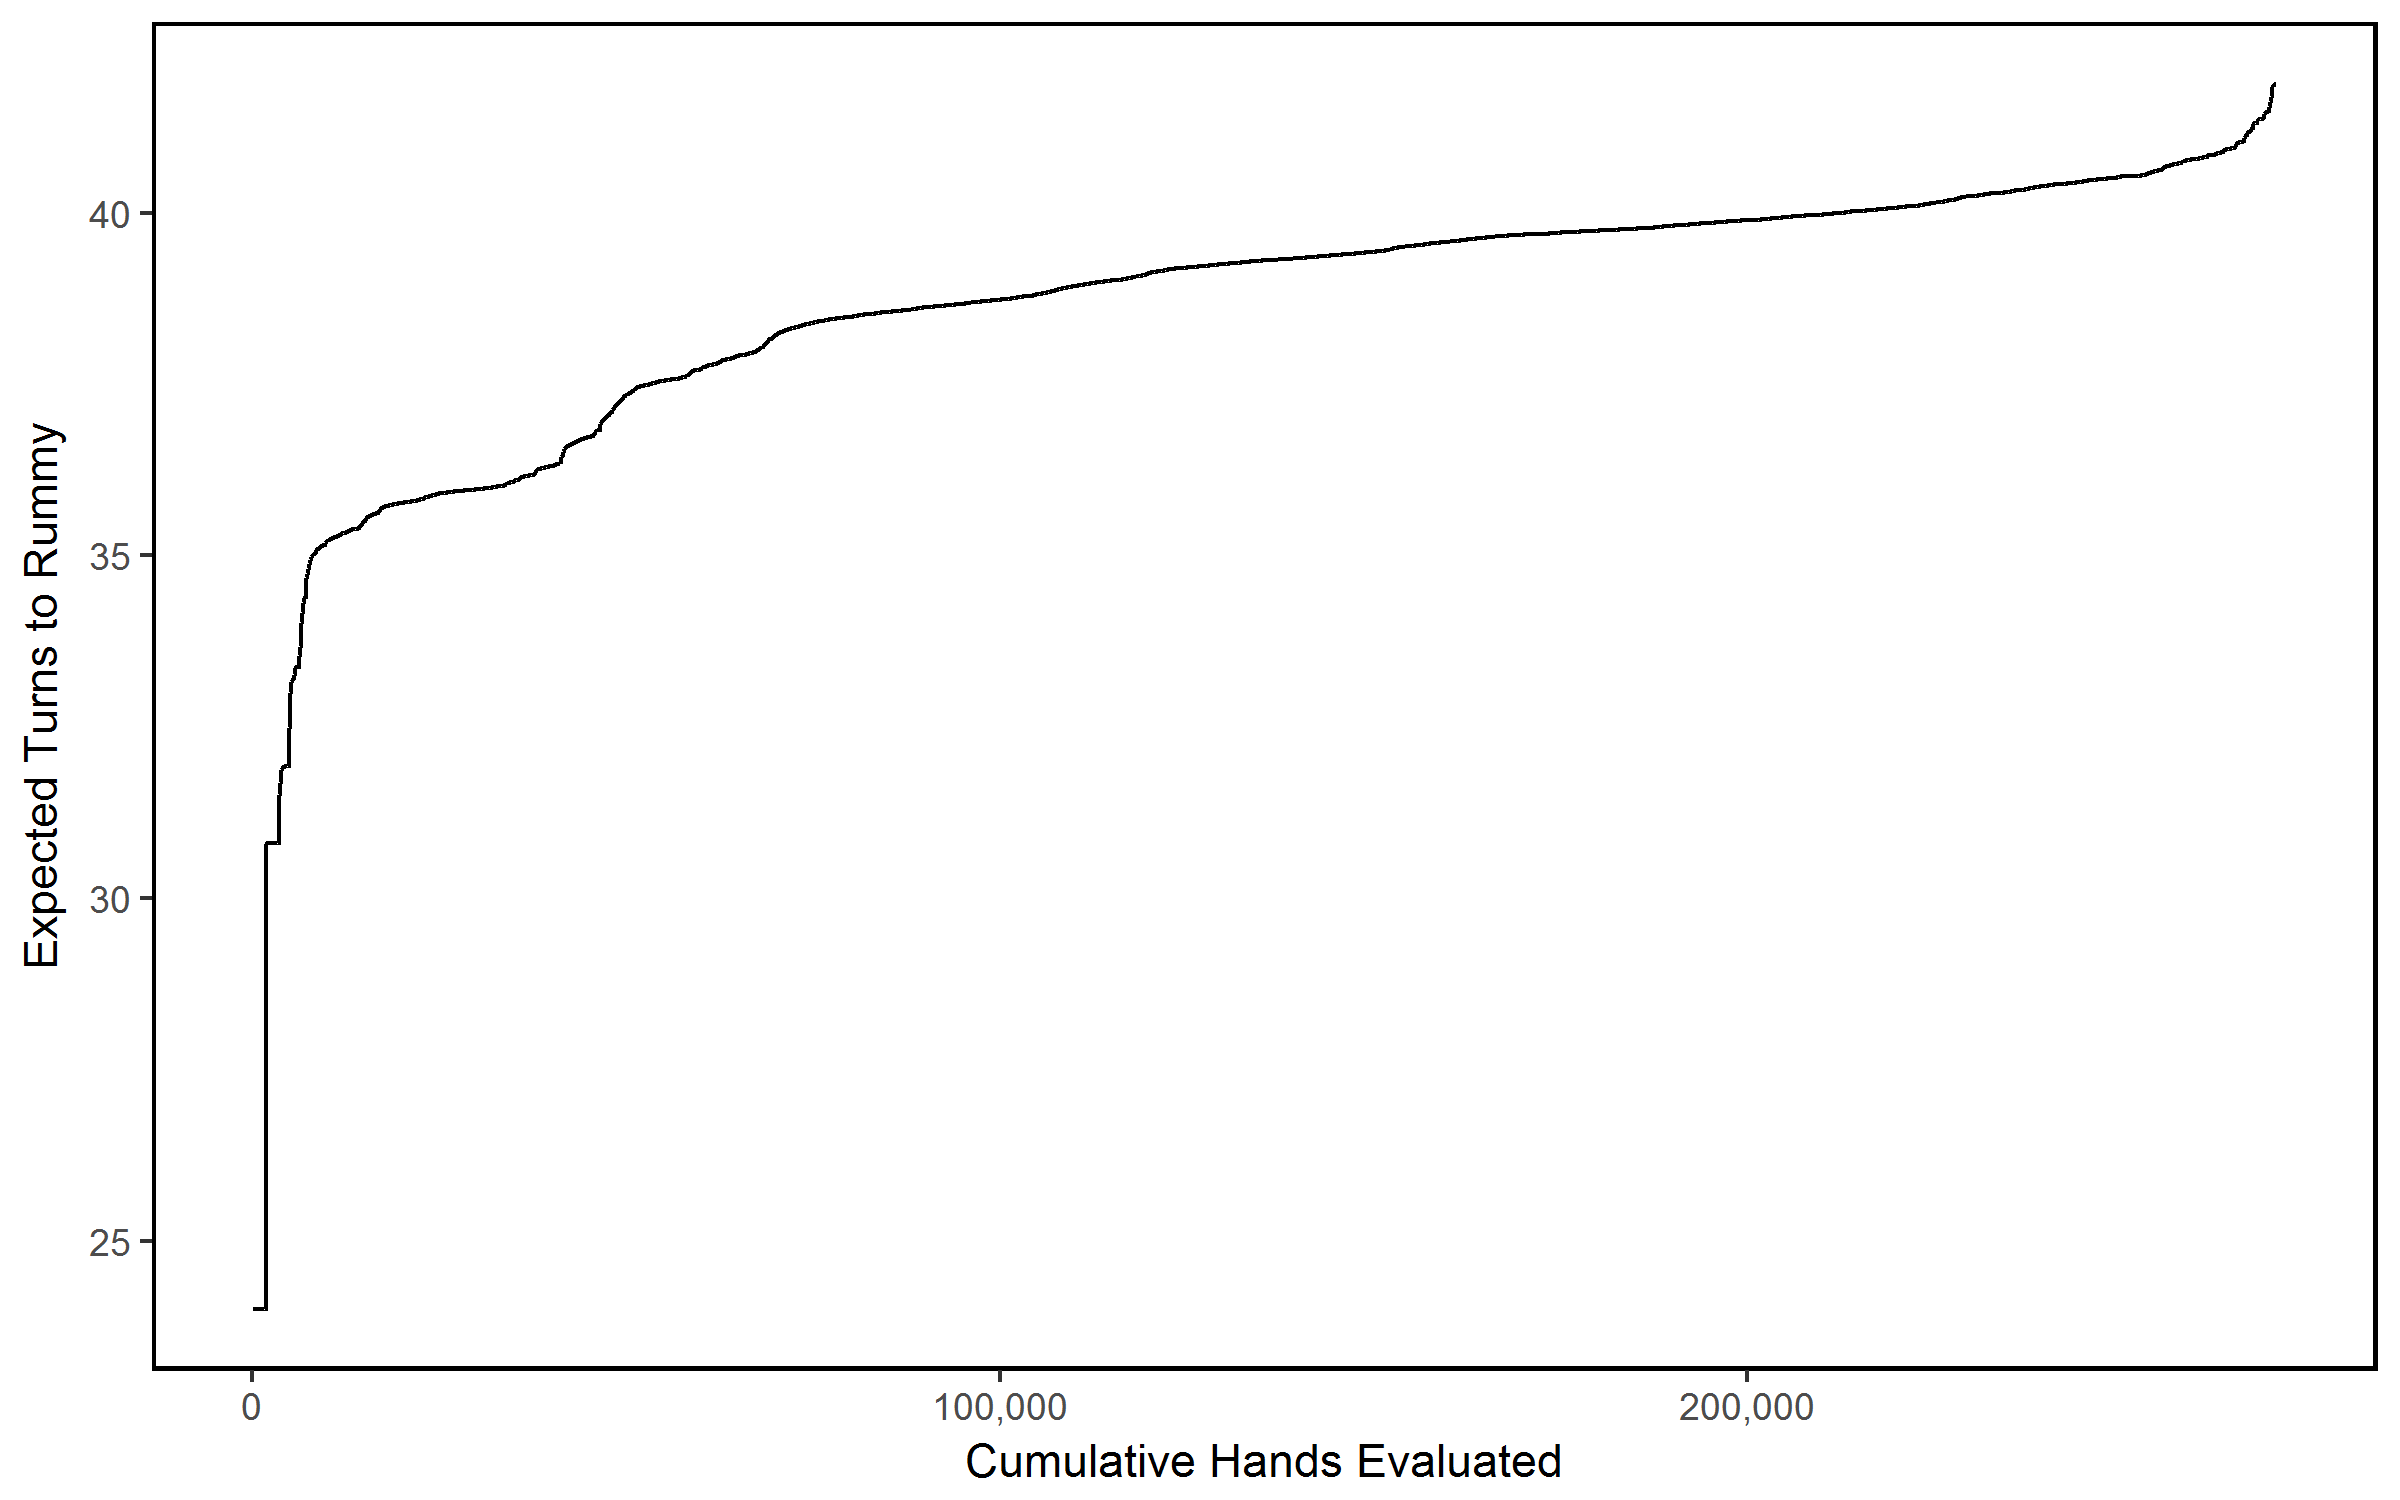
\includegraphics[width=\textwidth]{fig10.png}
\caption{Estimated E for 4-Card Rummy with Various Tolerances}\label{fig:10}
\end{figure}

\begin{figure}
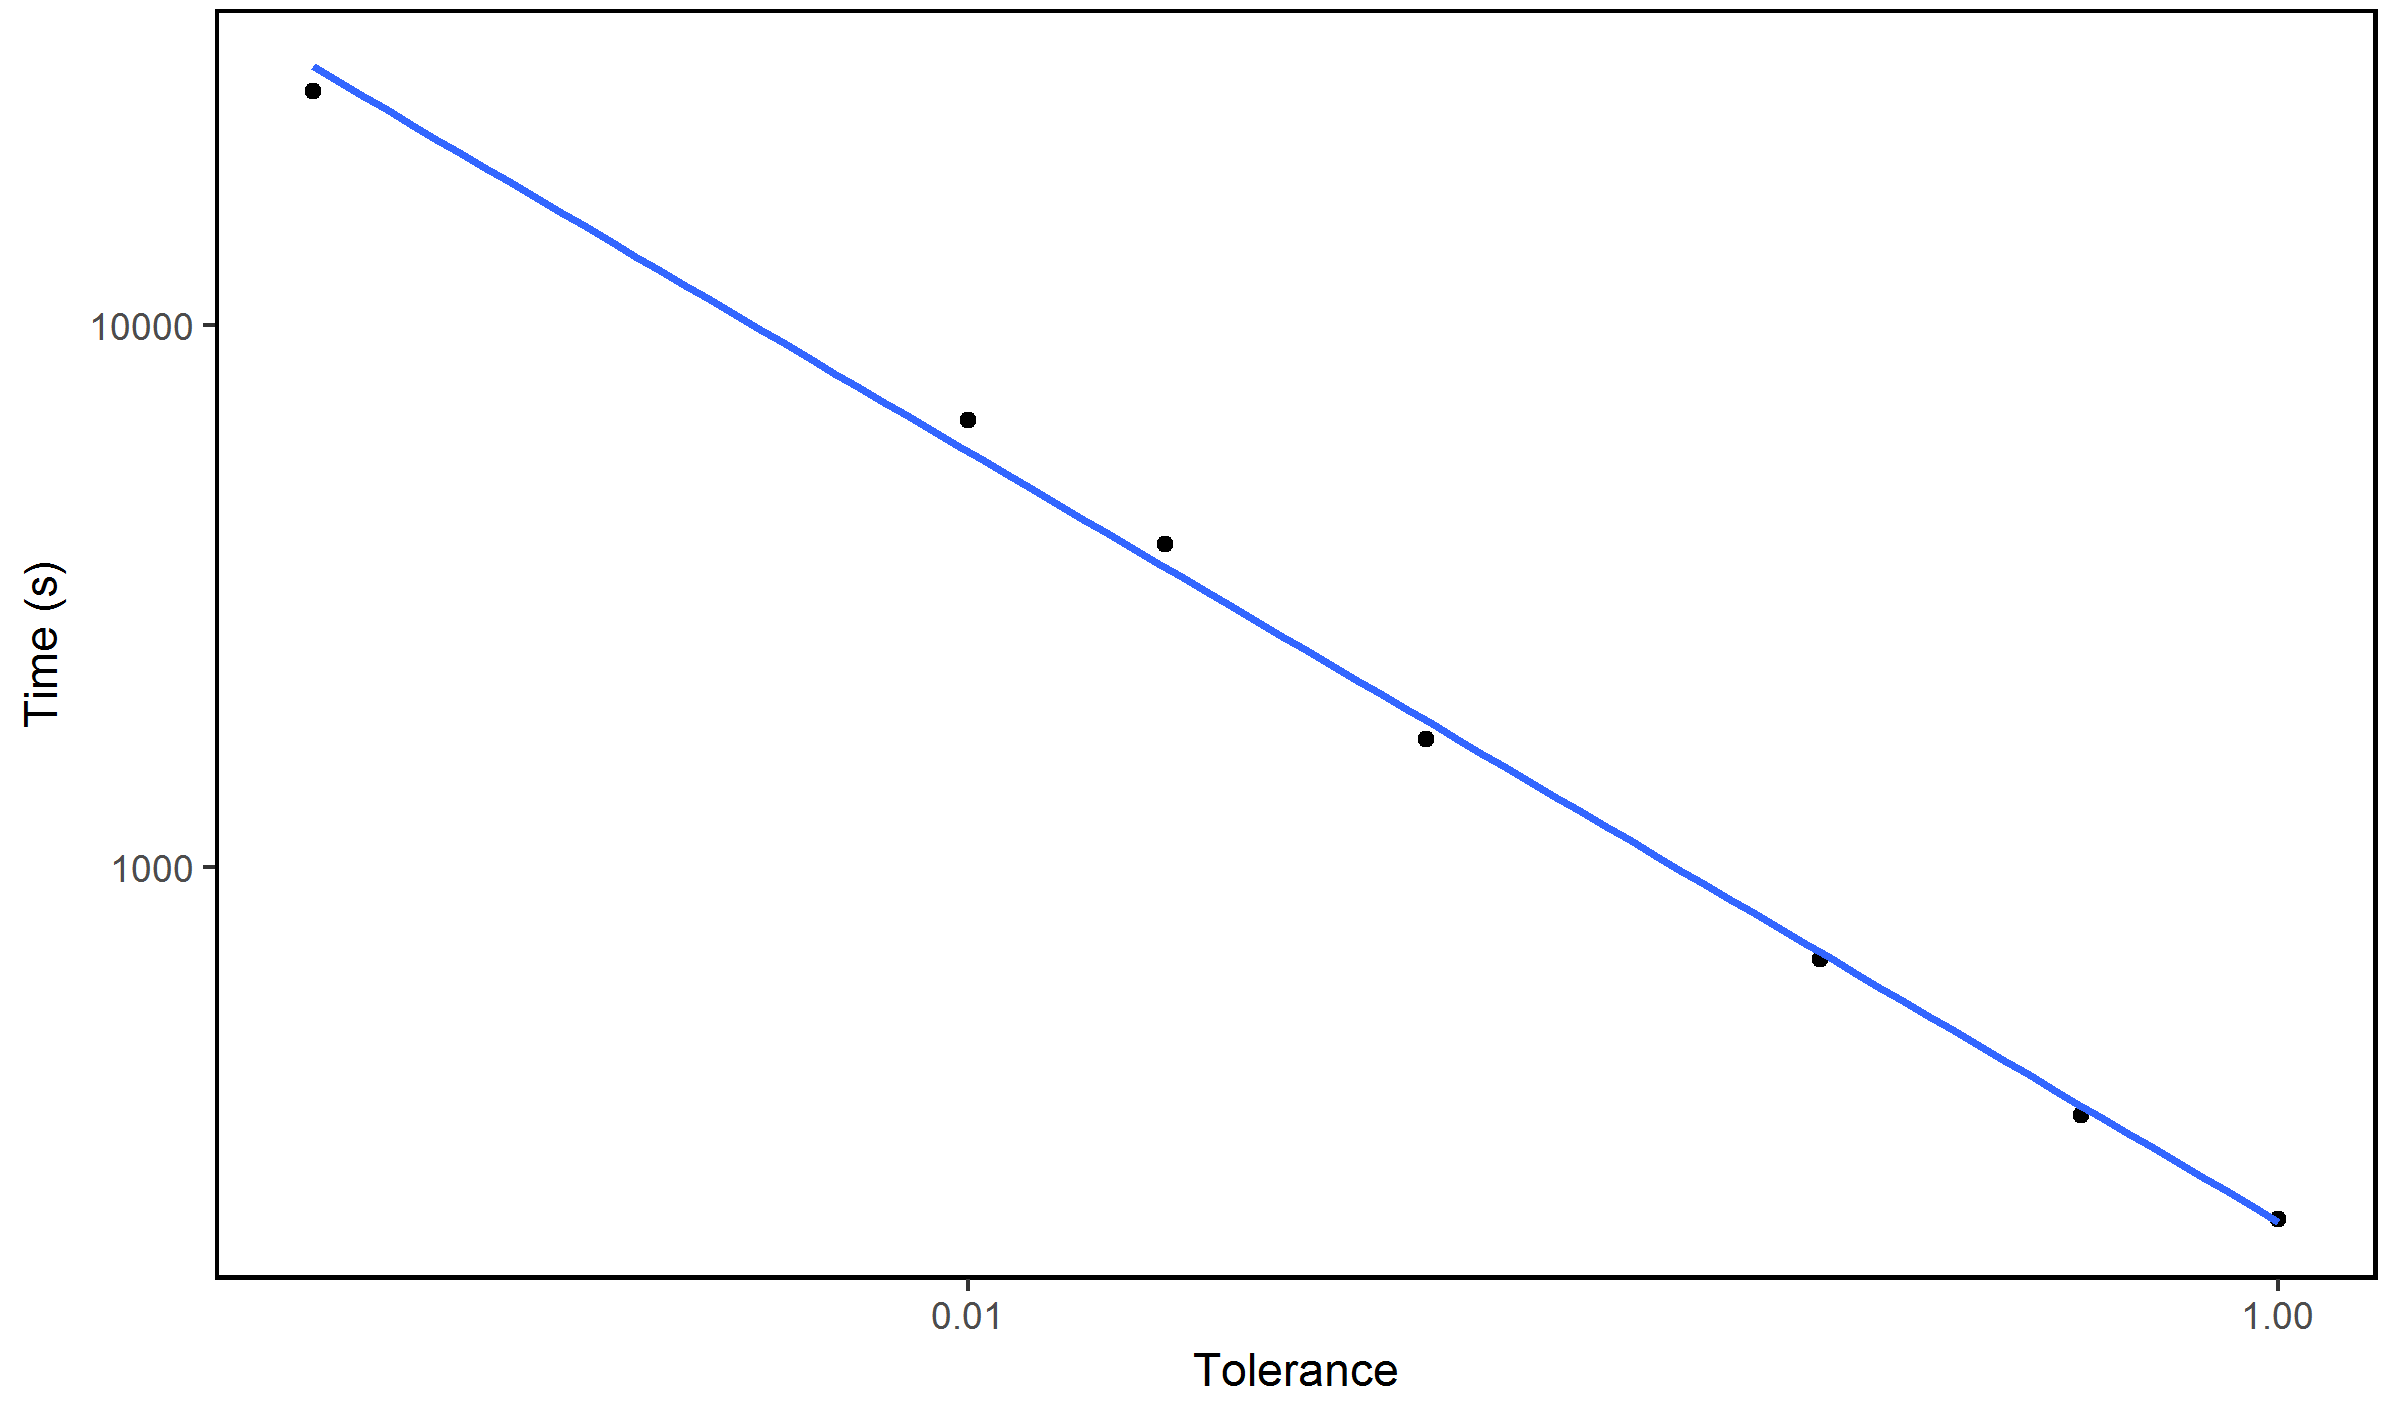
\includegraphics[width=\textwidth]{fig11.png}
\caption{Estimated E for 4-Card Rummy with Various Tolerances}\label{fig:11}
\end{figure}

In the end, we did run the 4-Card approximation with $t=0.001$. The results of this calculation are presented in Figure \ref{fig:10}. We may conclude that the true contours of the hand space for 4-Card Rummy deviate from this line by less than 0.001 turns for all hands. The calculation of these data was not as easy as the exponential model would lead us to expect, however - it took 27,108 seconds, or nearly 8 hours. Indeed, another regression (see Figure \ref{fig:11} based on 7 data points for 4-card Rummy indicates that the correct model for this more difficult approximation is

$$time = \beta * t^{-0.710}$$

with $\beta = 225$ in this case. In the previous model, the time required to calculate 3-Card Ace Low with full precision was approximately 1980 seconds, a time value which corresponds with the tolerance value $2.77*10^{-5}$. (Interestingly, the smallest difference between equivalence classes for that game is around $10^{-7}$, so this tolerance would not actually be sufficiently granular to collect all the results). Plugging this same tolerance value into the new model predicts that a complete explication of 4-Card Rummy with Aces Low would require $255 * 0.0000277^{-0.710} \approx 440000$ seconds $\approx 121$ hours. While this would not be impossible to achieve, it is certainly inconvenient and an order of magnitude longer than any other calculation performed for this project. Since the edge gained by a refinement of 0.001 turns is unlikely to change the outcome of a game, we can confidently call the Hand - E dictionary formed by the output of this approximation a satisficing solution for 4-Card Rummy with aces low. 

\section{Future Research}

\subsection{7-Card Rummy}

We still have not reached our goal of modeling a game that people might ever actually play, but with the completion of both 3-Card and 4-Card Rummy the ingredients are there. It is possible to imagine the outline of a scheme which could result in non-optimal but better-than-random policy function based on these data. Suppose we seed a list of all $\binom{52}{7}$ 7-card hands with adjusted versions of the known $E$ values for those hands which contain a 3-card or 4-card meld. The remaining hands may be more efficiently evaluated by their proximity to these halfway-complete hands. The implementation of this program would be highly involved, but in theory it could run in a reasonable time frame on higher-end hardware.

\subsection{Other Statistical Measures of a Given E}

All this time we have been calculating $E$, which for each hand is essentially the mean expected time until Rummy. But what is the variance around this mean? We could generate a computerized Rummy-playing agent which follows our policy function at all times and let it play a large number of games. The number of turns it requires to get to Rummy would hopefully follow some recognizable probability distribution with a mean at our calculated $E$, and we could then investigate the variance and standard deviation for that hand. With repetitions for many hands we could begin to come to some conclusions about the variance for all hands.

Once we have these data, more involved analysis of 3-card Rummy as a game in and of itself could be conducted (though the interest of such investigations may be limited). In theory, our optimized policy function represents a player with maximized skill. How does the function fare against a randomized opponent?   How much of the game is skill vs. luck? By generating agents with policy functions of varying efficacy (e.g. one for each approximate data set) and playing them off each other we might compare the completeness of their knowledge against their win/loss ratios and examine the correlation between knowledge completeness and victory.

\subsection{Programmatic Changes to More Accurately Simulate Actual Games}

We never made an attempt to correct our erroneous assumption that cards drawn are immediately replaced in the deck. Because of the efficiency of the new implementation, it might be possible to create a responsive program that will recalculate the $E$ for every hand after each discard in light of the longer time required to reintroduce that specific card to the set of possible draws. This would be especially feasible for 3-card Wrap, which requires a negligible amount of computation time.

However, this responsive paradigm will not scale to any sort of larger game. So another strategy might be to determine a static value-added model which can predetermine how much of a hand's 'goodness' or 'badness' is predicated on the presence of a certain card in the deck (and thus a certain future hand which becomes available). This method would have its own problems, chief among them the requirement of a huge amount of storage space for large games, and its mathematical validity is highly conjectural without further formal investigation.

\section{Appendix}

\subsection{C++ Code Sample - Hand.cpp}

In the early part of this semester, much time was spent re-writing the original python code into far faster C++ code. In order to create a flexible program, an object-oriented approach was used in which a single Hand object could be plugged into multiple calculations. Below is the code for that hand, which contains many of the relevant calculations. However, by itself the Hand object does nothing. The complete complement of other necessary files (including hand.h and, e.g., 3cardapprox.cpp) may be found at https://github.com/ChrisFinkle/RummySeniorProject.

\begin{scriptsize}
\begin{verbatim}
#include "hand.h"
#include <set>
#include <string>
#include <iostream>
using namespace std;

/*  Rummy hand class with methods designed for successive calculation of 
    expected times to Rummy. This class is multi-purpose; it can hold any
    number of cards (though in practice only 3 and 4 are useful). It can also
    have any definition of what is Rummy as desired; the isRummy function is
    defined in another program that uses Hand and passed in via the constructor,
    along with a point to an array containing all other possible hands, a map
    that serves as a 'guide' to said array, allowing fast lookup, knowledge
    of what size the hand is, and its cards.
*/
Hand::Hand(set<int> cards, int _size, Hand **_allHands, map<set<int>,int> *_idxs, bool (*_isRummy)(set<int>)){
    size = _size;
    isRummy = _isRummy;
    allHands = _allHands;
    idxs = _idxs;
    cardSet = cards;
    lockedIn = isRummy(cardSet);
    E = (isRummy(cardSet)) ? 0.0 : 500.0; //500 is a stand-in for a high, unknown value for hands which are not rummy
}

bool Hand::hasSameCards(set<int> compare){
    return compare==cardSet;
}

void Hand::assocHands(){
    for(int i=0; i<52; i++){
        set<int> newSet = cardSet;
        newSet.insert(i); //draw a random card
        if(newSet.size()>cardSet.size()){ //if card is not in your hand
            map<int, Hand*> m; //create map of outcomes by index of card discarded
            int j=0;
            for(set<int>::iterator it = cardSet.begin(); it!=cardSet.end(); ++it){
                newSet.erase(*it); //discard card
                m[j] = allHands[idxs->at(newSet)]; //search all hands for new hand, store ptr
                j++;
                newSet.insert(*it); //put the card back
            }
            futureHands[i] = m; //store map of outcomes
        }
    }
}


bool Hand::getLockedIn(){
    return lockedIn;
}

void Hand::lockIn(){
    lockedIn=true;
}

double Hand::evalE(){
    map<int, double> m;
    double sum = 0.0;
    //iterate over potential hands to draw
    for(map<int, map<int,Hand*>>::iterator it = futureHands.begin(); it!=futureHands.end(); ++it){
        map<int,Hand*> n = it->second; //possible post-discard outcomes
        //among locked-in future hands, if hand not yet stored in m or if hand is lower than value
        //currently stored in m under the drawn card, stores E in m.
        for(map<int,Hand*>::iterator it2 = n.begin(); it2!=n.end(); ++it2){
            if(it2->second->getLockedIn() && (m.count(it->first)==0 || m[it->first]>it2->second->getE())){
                m[it->first]=it2->second->getE();
            }
        }
    }
    //adds up all Es in accordance with Bellman sum
    for(map<int, double>::iterator it3 = m.begin(); it3!=m.end(); ++it3){
        sum += it3->second;
    }
    //if any future hands locked in, calculate final value in accordance w/ Bellman sum
    if(m.size()>0){
        E = (sum+52.0-(float)size)/(float)m.size();
    }
    return E;
}

double Hand::getE(){
    return E;
}

string Hand::prettyPrintHand(){
    string st = "";
    for(set<int>::iterator it = cardSet.begin(); it!=cardSet.end(); ++it){
        string s = "X";
        if(*it%4==0){s="C";} //Clubs
        else if(*it%4==1){s="D";} //Diamonds
        else if(*it%4==2){s="H";} //Hearts
        else if(*it%4==3){s="S";} //Spades
        string v = "X";
        if(*it/4==0){v="A";} //Ace
        else if(*it/4==1){v="2";}
        else if(*it/4==2){v="3";}
        else if(*it/4==3){v="4";}
        else if(*it/4==4){v="5";}
        else if(*it/4==5){v="6";}
        else if(*it/4==6){v="7";}
        else if(*it/4==7){v="8";}
        else if(*it/4==8){v="9";}
        else if(*it/4==9){v="T";} //Ten
        else if(*it/4==10){v="J";} //Jack
        else if(*it/4==11){v="Q";} //Queen
        else if(*it/4==12){v="K";} //King
        st = st + v;
        st = st + s;
        st = st + " ";
    }
    return st;
}

bool Hand::getIsRummy(){
    return isRummy(cardSet); //function pointer
}

//resets E without resetting hand associations; used in batch approximations
void Hand::reset(){
    lockedIn = false;
    E = (isRummy(cardSet)) ? 0.0 : 500.0;
}
\end{verbatim}
\end{scriptsize}

{\setlength{\parindent}{0 cm}
\subsection{Summary of Results for 3-Card Continuity Rummy}

$\texttt{312 hands like A$\clubsuit$ A$\diamondsuit$ 2$\clubsuit$ with E = 12.2500000000}$

$\texttt{312 hands like A$\clubsuit$ A$\diamondsuit$ 3$\clubsuit$ with E = 14.2916666667}$

$\texttt{104 hands like A$\clubsuit$ 2$\clubsuit$ 4$\clubsuit$ with E = 15.0340909091}$

$\texttt{312 hands like A$\clubsuit$ 2$\clubsuit$ 4$\diamondsuit$ with E = 15.1825757576}$

$\texttt{1768 hands like A$\clubsuit$ 2$\clubsuit$ 3$\diamondsuit$ with E = 15.2289772727}$

$\texttt{624 hands like A$\clubsuit$ A$\diamondsuit$ 3$\heartsuit$ with E = 15.4648516414}$

$\texttt{1560 hands like A$\clubsuit$ A$\diamondsuit$ 5$\clubsuit$ with E = 15.4671717172}$

$\texttt{312 hands like A$\clubsuit$ A$\diamondsuit$ 5$\heartsuit$ with E = 15.4672327718}$

$\texttt{312 hands like A$\clubsuit$ A$\diamondsuit$ 4$\clubsuit$ with E = 15.4728488282}$

$\texttt{312 hands like A$\clubsuit$ A$\diamondsuit$ 2$\heartsuit$ with E = 15.4728992646}$

$\texttt{52 hands like A$\clubsuit$ 3$\clubsuit$ 5$\clubsuit$ with E = 15.9763986014}$

$\texttt{312 hands like A$\clubsuit$ 2$\diamondsuit$ 4$\diamondsuit$ with E = 17.0074215715}$

$\texttt{312 hands like A$\clubsuit$ 3$\clubsuit$ 5$\diamondsuit$ with E = 17.0732305628}$

$\texttt{312 hands like A$\clubsuit$ 3$\clubsuit$ 6$\diamondsuit$ with E = 17.0737070109}$

$\texttt{520 hands like A$\clubsuit$ 3$\clubsuit$ 7$\clubsuit$ with E = 17.0751942232}$

$\texttt{312 hands like A$\clubsuit$ 3$\clubsuit$ 7$\diamondsuit$ with E = 17.0752304967}$

$\texttt{104 hands like A$\clubsuit$ 3$\clubsuit$ 6$\clubsuit$ with E = 17.0953850796}$

$\texttt{156 hands like A$\clubsuit$ 2$\diamondsuit$ 3$\clubsuit$ with E = 17.1010958053}$

$\texttt{312 hands like A$\clubsuit$ 2$\diamondsuit$ 3$\heartsuit$ with E = 18.0920515788}$

$\texttt{624 hands like A$\clubsuit$ 2$\diamondsuit$ 4$\heartsuit$ with E = 18.1338076896}$

$\texttt{312 hands like A$\clubsuit$ 2$\diamondsuit$ 5$\clubsuit$ with E = 18.1394661776}$

$\texttt{624 hands like A$\clubsuit$ 2$\diamondsuit$ 5$\heartsuit$ with E = 18.1401919365}$

$\texttt{624 hands like A$\clubsuit$ 2$\diamondsuit$ 8$\clubsuit$ with E = 18.1437838885}$

$\texttt{312 hands like A$\clubsuit$ 2$\diamondsuit$ 7$\diamondsuit$ with E = 18.1437859037}$

$\texttt{624 hands like A$\clubsuit$ 2$\diamondsuit$ 7$\heartsuit$ with E = 18.1438418627}$

$\texttt{312 hands like A$\clubsuit$ 2$\diamondsuit$ 7$\clubsuit$ with E = 18.1438635222}$

$\texttt{624 hands like A$\clubsuit$ 2$\diamondsuit$ 6$\heartsuit$ with E = 18.1440412502}$

$\texttt{312 hands like A$\clubsuit$ 2$\diamondsuit$ 6$\clubsuit$ with E = 18.1443161989}$

$\texttt{312 hands like A$\clubsuit$ 2$\diamondsuit$ 6$\diamondsuit$ with E = 18.1445854036}$

$\texttt{312 hands like A$\clubsuit$ 3$\diamondsuit$ 5$\heartsuit$ with E = 18.1487838203}$

$\texttt{312 hands like A$\clubsuit$ 3$\diamondsuit$ 6$\clubsuit$ with E = 18.1540668969}$

$\texttt{624 hands like A$\clubsuit$ 3$\diamondsuit$ 6$\heartsuit$ with E = 18.1540684957}$

$\texttt{312 hands like A$\clubsuit$ 4$\diamondsuit$ 7$\heartsuit$ with E = 18.1558105415}$

$\texttt{156 hands like A$\clubsuit$ 4$\diamondsuit$ 7$\clubsuit$ with E = 18.1559882568}$

$\texttt{312 hands like A$\clubsuit$ 3$\diamondsuit$ 7$\diamondsuit$ with E = 18.1579439075}$

$\texttt{312 hands like A$\clubsuit$ 3$\diamondsuit$ 8$\diamondsuit$ with E = 18.1583001130}$

$\texttt{624 hands like A$\clubsuit$ 3$\diamondsuit$ 8$\heartsuit$ with E = 18.1583682569}$

$\texttt{624 hands like A$\clubsuit$ 3$\diamondsuit$ 7$\heartsuit$ with E = 18.1583950372}$

$\texttt{312 hands like A$\clubsuit$ 3$\diamondsuit$ 8$\clubsuit$ with E = 18.1584902829}$

$\texttt{312 hands like A$\clubsuit$ 3$\diamondsuit$ 7$\clubsuit$ with E = 18.1587980145}$

$\texttt{312 hands like A$\clubsuit$ 4$\diamondsuit$ 8$\diamondsuit$ with E = 18.1605346891}$

$\texttt{312 hands like A$\clubsuit$ 4$\diamondsuit$ 9$\clubsuit$ with E = 18.1607829051}$

$\texttt{624 hands like A$\clubsuit$ 4$\diamondsuit$ 8$\heartsuit$ with E = 18.1608152911}$

$\texttt{312 hands like A$\clubsuit$ 4$\diamondsuit$ 8$\clubsuit$ with E = 18.1608372793}$

$\texttt{312 hands like A$\clubsuit$ 4$\diamondsuit$ 9$\heartsuit$ with E = 18.1608457260}$

$\texttt{52 hands like A$\clubsuit$ 5$\clubsuit$ 9$\clubsuit$ with E = 18.1651663447}$

$\texttt{156 hands like A$\clubsuit$ 5$\diamondsuit$ 9$\clubsuit$ with E = 18.1653875144}$

$\texttt{312 hands like A$\clubsuit$ 5$\clubsuit$ 9$\diamondsuit$ with E = 18.1654198678}$

$\texttt{312 hands like A$\clubsuit$ 5$\diamondsuit$ 9$\heartsuit$ with E = 18.1654807138}$

$\texttt{156 hands like A$\clubsuit$ 3$\diamondsuit$ 5$\clubsuit$ with E = 18.1757181485}$

$\texttt{312 hands like A$\clubsuit$ 2$\diamondsuit$ 5$\diamondsuit$ with E = 18.1836742219}$

$\texttt{312 hands like A$\clubsuit$ 2$\diamondsuit$ 4$\clubsuit$ with E = 18.1838851671}$

$\texttt{312 hands like A$\clubsuit$ 3$\diamondsuit$ 6$\diamondsuit$ with E = 18.1979628021}$

$\texttt{312 hands like A$\clubsuit$ 4$\clubsuit$ 7$\diamondsuit$ with E = 18.1987828975}$

$\texttt{52 hands like A$\clubsuit$ 4$\clubsuit$ 9$\clubsuit$ with E = 18.2034678729}$

$\texttt{104 hands like A$\clubsuit$ 4$\clubsuit$ 8$\clubsuit$ with E = 18.2036285598}$

$\texttt{312 hands like A$\clubsuit$ 4$\clubsuit$ 8$\diamondsuit$ with E = 18.2044667946}$

$\texttt{156 hands like A$\clubsuit$ 4$\clubsuit$ 9$\diamondsuit$ with E = 18.2044988437}$

$\texttt{52 hands like A$\clubsuit$ 4$\clubsuit$ 7$\clubsuit$ with E = 18.2442485400}$

\subsection{Summary of Results for Approximations of 3-Card Rummy with Aces Low}

When the tolerance is set to 1.0 the results are as follows:

$\texttt{240 hands like 2$\clubsuit$ 2$\diamondsuit$ 3$\clubsuit$ with E = 12.2500000000}$

$\texttt{216 hands like A$\clubsuit$ 3$\clubsuit$ 3$\diamondsuit$ with E = 14.2916666667}$

$\texttt{3912 hands like A$\clubsuit$ A$\diamondsuit$ 3$\clubsuit$ with E = 14.8750000000}$

$\texttt{564 hands like A$\clubsuit$ A$\diamondsuit$ 2$\clubsuit$ with E = 15.7500000000}$

$\texttt{2116 hands like A$\clubsuit$ A$\diamondsuit$ 2$\heartsuit$ with E = 17.0207896270}$

$\texttt{4192 hands like A$\clubsuit$ A$\diamondsuit$ K$\clubsuit$ with E = 17.3911492987}$

$\texttt{8180 hands like A$\clubsuit$ 2$\clubsuit$ Q$\clubsuit$ with E = 18.2932809113}$

$\texttt{2488 hands like A$\clubsuit$ 2$\diamondsuit$ 3$\heartsuit$ with E = 18.7476800197}$

$\texttt{96 hands like A$\clubsuit$ 2$\diamondsuit$ K$\clubsuit$ with E = 19.3163153484}$

\smallskip
For comparison, these are the results when the tolerance is 0.5:

$\texttt{240 hands like 2$\clubsuit$ 2$\diamondsuit$ 3$\clubsuit$ with E = 12.2500000000}$

$\texttt{216 hands like A$\clubsuit$ 3$\clubsuit$ 3$\diamondsuit$ with E = 14.2916666667}$

$\texttt{1752 hands like A$\clubsuit$ A$\diamondsuit$ 3$\clubsuit$ with E = 14.8750000000}$

$\texttt{2184 hands like A$\clubsuit$ A$\diamondsuit$ 2$\clubsuit$ with E = 15.4731867284}$

$\texttt{420 hands like A$\clubsuit$ 3$\clubsuit$ 5$\clubsuit$ with E = 15.9763986014}$

$\texttt{120 hands like A$\clubsuit$ 2$\diamondsuit$ 2$\heartsuit$ with E = 16.3252494553}$

$\texttt{1484 hands like A$\clubsuit$ A$\diamondsuit$ 3$\heartsuit$ with E = 17.0145782073}$

$\texttt{672 hands like A$\clubsuit$ A$\diamondsuit$ 2$\heartsuit$ with E = 17.2325884407}$

$\texttt{696 hands like A$\clubsuit$ 2$\clubsuit$ 4$\diamondsuit$ with E = 17.6765799652}$

$\texttt{6972 hands like A$\clubsuit$ 2$\clubsuit$ 3$\diamondsuit$ with E = 18.1432355981}$

$\texttt{6424 hands like A$\clubsuit$ 2$\diamondsuit$ 3$\heartsuit$ with E = 18.4305322314}$

$\texttt{824 hands like A$\clubsuit$ 2$\diamondsuit$ 5$\diamondsuit$ with E = 18.8536850047}$

\newpage

\begin{center}\section*{References}\end{center}
\addcontentsline{toc}{section}{References}

Bellman, Richard E. (1957). Dynamic Programming. Princeton, NJ: Princeton University Press. 
\\
\\
Gibson, Walter. (1974). Hoyle’s Modern Encyclopedia of Card Games. New York: Doubleday. 
\\
\\
Kotnik, Clifford, $\&$ Kalita, Jugal (2003). The significance of temporal-difference learning in selfplay training td-rummy versus evo-rummy. In ICML (pp. 369-375). 
\\
\\
Parlett, David. (1978). The Penguin Book of Card Games. London: Penguin 
\\
\\
Saeed, Ghahramani. (2005) Fundamentals of Probability with Stochastic Processes. 3rd Edition.  Upper Saddle River, NJ: Pearson Education.
}
\end{document}